\documentclass[12pt,letterpaper]{article}

\usepackage[pages=all, color=black, position={current page.south}, placement=bottom, scale=1, opacity=1, vshift=5mm]{background}
%\SetBgContents{
%	\tt This work is shared under a \href{https://creativecommons.org/licenses/by-sa/4.0/}{CC BY-SA 4.0 license} unless otherwise noted
%}      % copyright

\usepackage[margin=1in]{geometry} % full-width

% AMS Packages
\usepackage{amsmath}
\usepackage{amsthm}
\usepackage{amssymb}
\usepackage{lato}

% Unicode
\usepackage[utf8]{inputenc}
\usepackage{hyperref}
\hypersetup{
	unicode,
%	colorlinks,
%	breaklinks,
%	urlcolor=cyan, 
%	linkcolor=blue, 
	pdfauthor={Author One, Author Two, Author Three},
	pdftitle={A simple article template},
	pdfsubject={A simple article template},
	pdfkeywords={article, template, simple},
	pdfproducer={LaTeX},
	pdfcreator={pdflatex}
}

% Vietnamese
%\usepackage{vntex}

% Natbib
%\usepackage[sort&compress,numbers,square]{natbib}
%\bibliographystyle{mplainnat}

% Theorem, Lemma, etc
\theoremstyle{plain}
\newtheorem{theorem}{Theorem}
\newtheorem{corollary}[theorem]{Corollary}
\newtheorem{lemma}[theorem]{Lemma}
\newtheorem{claim}{Claim}[theorem]
\newtheorem{axiom}[theorem]{Axiom}
\newtheorem{conjecture}[theorem]{Conjecture}
\newtheorem{fact}[theorem]{Fact}
\newtheorem{hypothesis}[theorem]{Hypothesis}
\newtheorem{assumption}[theorem]{Assumption}
\newtheorem{proposition}[theorem]{Proposition}
\newtheorem{criterion}[theorem]{Criterion}
\theoremstyle{definition}
\newtheorem{definition}[theorem]{Definition}
\newtheorem{example}[theorem]{Example}
\newtheorem{remark}[theorem]{Remark}
\newtheorem{problem}[theorem]{Problem}
\newtheorem{principle}[theorem]{Principle}

\usepackage{graphicx, color}
\usepackage{booktabs}
\graphicspath{{fig/}}

\usepackage[square,sort,comma,numbers]{natbib}
\bibliographystyle{apalike}
\bibpunct{(}{)}{,}{a}{,}{,}


%\usepackage[linesnumbered,ruled,vlined,commentsnumbered]{algorithm2e} % use algorithm2e for typesetting algorithms
\usepackage{algorithm, algpseudocode} % use algorithm and algorithmicx for typesetting algorithms
\usepackage{mathrsfs} % for \mathscr command


% Author info
\title{Challenges of Incorporating Rotation Information into Crop Insurance Rates}
\author{Author One$^1$\thanks{Author One was partially supported by Grant XXX} \and Author Two$^2$ \and Author Three$^1$}

\date{
	$^1$Organization 1 \\ \texttt{\{auth1, auth3\}@org1.edu}\\%
	$^2$Organization 2 \\ \texttt{auth3@inst2.edu}\\[2ex]%
%	\today
}

\begin{document}
	\maketitle
	
	\begin{abstract}
		We investigate how long-term crop rotation patterns affect corn yields. The research is motivated by an interest in incorporating farm-level conservation practices, such as crop rotations, into crop insurance rates. These practices are believed to mitigate yield risk and provide agroecological benefits for farm production, particularly in the face of adverse weather events. However, challenges exist in developing a rating system due to the nonlinear relationship between yields and diversity indices.

    This study employs linear fixed effects models to quantify the magnitude of the relationship between yields and rotational complexity, accounting for land quality, and modeling the conditional first and second moments of the yield distribution. Data sources include the Scalable Satellite-Based Crop Yield Mapper (SCYM) and Quantile loss Domain Adversarial Neural Networks (QDANN) yield data, the Rotational Complexity Index (RCI), field-level crop data (CDL), and weather variables (PRISM). QDANN has a higher reported accuracy than SCYM.

    Key findings suggest that corn monoculture is not the most productive pattern in terms of either the mean or variance of corn yields. We find a handful of rotations that outperform monoculture. However, transitioning from monoculture to a corn-soy rotation most often lowers yields until a well-designed rotation plan is established. We argue that the majority of farmers engage in simple rotation patterns; our dataset shows that 51\% of fields follow a perfect corn/soy rotation, 8\% engage in corn monoculture, while the remaining 41\% correspond to other patterns. Future work will include more complex rotation patterns, such as rotations with Wheat or Alfalfa, and cover crops.

    %High-performing sequences typically feature a recent soy rotation (years 1 or 2), no consecutive soy years, and a low impact from older crops (within the first three years). A perfect corn/soy rotation, while positive, has non-significant effects on yields and reduces yield variance. Later soybean rotations and shorter gaps between soy harvests have more positive and significant effects on yields. Conversely, more and less spaced-out soy harvests show negative and significant effects on corn yields. The analysis reveals that only a limited number of rotation sequences outperform corn monoculture in achieving higher mean yields and lower yield variance.

    %We identify four key indicators that account for variations in corn yield moments: Soy Lag (number of lagged periods since the most recent soy harvest), Consecutive soy years (dummy for two or more consecutive soy harvests), Soy gap (minimum number of years between two soy harvests), and Number of soy harvests across six years. These variables are used to construct a rotation score, which summarizes rotation patterns and allows for the prediction of yields, serving as a tool for causal identification of the effect of shifting rotations on yield outcomes.
	\end{abstract}

	%\tableofcontents
    \newpage
	
	\section{Introduction}
	\label{sec:intro}

    This article investigates the relationship between longer-term rotation patterns and crop yields. 
	
	\emph{Research Question}: How do long-term crop rotation patterns affect corn yields?
    
    \emph{Method}: We use linear fixed effects models to quantify the magnitude of the relationship between yields and rotational complexity.
    
    \emph{Data}: Yield (biomass) data from \cite{lobell2015} (SCYM) and \cite{Ma2024} (QDANN), Rotational complexity index, from \cite{socolar2021}, field-level crops (CDL), and weather variables (PRISM).
    
    \emph{Results}: The effect of rotations on yields depends critically on their timing; later soybean rotations and shorter gaps between soy harvests have more positive and significant effects on yields.
    
    However, more and less spaced-out soy harvests have negative and significant effects on corn yields.
	
	\subsection{Preliminaries}
	\label{sec:pre}
	
	Interest in incorporating farm-level conservation practices into crop insurance rates?
        \begin{itemize}
            \item Cover cropping
            \item No till farming
            \item Crop rotations (corn and soybeans plus other crops)
        \end{itemize}
    
    These practices are thought to reduce yield risk, but may adversely affect short-term yields and farmer premium rates through their APH.
    
    Potentially reduce practice adoption incentives
    
\subsection{Rotational Complexity Index (RCI)\label{subsec:rci}}	
Increased rotation shown to have agroecological benefits for farm production, particularly in the face of adverse weather events \citep{socolar2021, burchfield2024}. Rotations help maintain soil organic carbon and fertility and reduce yield variability \citep{wu2025}. 


Still, this effect is conditional on soil characteristics (higher yield boost in lower productivity areas).
    
    Corn and soy rotations are the most prevalent in the US Midwest
    
    Challenges exist from a rating perspective for incorporating crop rotations into the rates.
	
There are several ways to measure ecological diversity
    \begin{enumerate}
        \item Rotational Complexity Index (RCI)
        \item Landscape Diversity Index
        \item Entropy-based measures
        \item Diversity indexes (weighted average of each number of crops)
    \end{enumerate}
    
Values of these indices can be incorporated into the rating system
    
    However, yields and yield risk are not a linear function of diversity indices, which presents a challenge for rating.
	
	Objectives:

    \begin{itemize}
        \item Show that RCI has a nonlinear effect on yield and yield risk.
        \item Determine identifiable indicators in a 6-year corn soy. rotation that affect yield and yield risk.
        \item Develop a rotation score and rank 6-year rotations using score.
    \end{itemize}

\subsection{Data Description\label{sec:data}}

\textbf{Scalable Satellite-Based Crop Yield Mapper (SCYM) yield data}:  a method and system developed by researchers \citep{lobell2015} for estimating crop yields using satellite data across large agricultural areas without needing ground-based yield measurements for calibration. It relies on a large number of crop model simulations over a range of soil, climate, and management conditions daily to train a statistical model at a pixel level, which is used to predict field-level biomass that can be converted to yields.
    
\textbf{Quantile Loss Domain Adversarial Neural Networks (QDANN) yield data}: QDANN is a machine-learning approach that combines three ideas:
    \begin{itemize}
        \item Domain-Adversarial Neural Networks (DANN).
        \item Quantile regression (via quantile loss / pinball loss).
        \item Distributionally robust prediction across domains.
    \end{itemize}

QDANN is mainly used to predict an outcome in a target domain where labels are scarce or unavailable, and where the researcher cares about uncertainty or the full conditional distribution, not just the mean. \citep{Ma2024} uses county-level yields and field-level data to train a neural network, which is then used to predict field-level yields via a technique called \textit{Unsupervised Domain Adaptation}. UDA is a machine-learning setting that trains a model on labeled data from a source domain and adapts it to a target domain with no labels, assuming the task remains the same, but the data distributions differ. The goal is to make predictions that work well in the target domain despite distribution shifts. Reported accuracy for QDANN is higher than that of SCYM (35\% for SCYM versus 48\% for QDANN at a field level).

Crop data comes from the Cropland Data Layer (CDL), a geospatial dataset of annual crop-specific land cover for the United States produced by the National Agricultural Statistics Service (NASS) of the U.S. Department of Agriculture (USDA). It provides raster maps showing where different crops and other land cover types are located each year, based on satellite imagery and agricultural reference data. We use yearly CDL data from 2003 to 2022. Each pixel represents a location on the ground and is classified into a crop or land cover category at 30m resolution. This information is used to calculate the Rotational Complexity Index (RCI).

Weather data (minimum and maximum temperature, vapor-pressure deficit, precipitation, and cumulative growing degreee-days come from GRIDMET, the Gridded Surface Meteorological dataset, \citep{Abatzoglou2013}, a high-resolution daily climate and weather dataset widely used in environmental, ecological, agricultural, hydrological, and climate research.

Climate water deficit data comes from TerraClimate \citep{Abatzoglou2018}, a widely used global gridded climate dataset that provides monthly-resolved climate data and derived water-balance variables at high spatial resolution (4 km) for land surfaces around the world, spanning from the late 1950s to the present. TerraClimate covers nearly all land areas on Earth (from about 90$^{\circ}$ N to 90$^{\circ}$ S) and provides consistent climate information in a spatial grid.

Finally, we use soil data from gSSURGO, the Gridded Soil Survey Geographic Database, a digital soil data product created by the U.S. Department of Agriculture’s Natural Resources Conservation Service (USDA-NRCS). It provides high-resolution, rasterized soil information across large areas of the United States, making detailed soil properties easier to use in mapping and environmental modeling. From this database, we get the NCCPI, National Commodity Crop Productivity Index for corn and soybeans (weighted average) for major earthy components; the Root zone (commodity crop) available water storage estimate, expressed in milimeters, defined as the volume of plant available water that the soil can store within the root zone based on all map unit earthy major components (weighted average); And the Soil organic carbon stock estimate (SOC) in standard zone 4 (0-100 cm depth). The concentration of organic carbon present in the soil is expressed in grams per square meter to a depth of 100 cm. 
    
%Both models use Landsat data as their main input, along with Gridmet data to calibrate yield models at a 30m resolution.
    
	
\section{Methods\label{sec:methods}}

\cite{Just1979} propose a flexible stochastic specification that allows researchers to independently estimate how inputs affect both the average yield and the associated risk. They demonstrate that common models often overstate the precision of their results and fail to account for inputs that may actually reduce production risk. 

Each year, a farmer decides which crop $c$ to grow ($c\in 
\{corn,soy\}$) on the basis of their expected profits, which depend mostly on the expected harvest price and their expected yields. This decision is also motivated by intrinsic factors not observable by a researcher; these elements are usually called ``management ability''. To control for these idiosyncratic factors, we use repeated observations from the same field across years to estimate a fixed-effects model with field IDs as controls. Similarly, we want to control for the presence of (linear) time trends; therefore, we also include year fixed-effects.

We model the conditional moments from the yield distribution as:
\begin{equation*}
yields_{it}=seq_{it}+W_{it}\beta_{it}+\lambda_{i}+\gamma_{t}+\varepsilon_{it}
\end{equation*}

Where:
\begin{description}
    \item[$yields_{it}$]: corn yields (in bushels per acre) of field $i$ in year$t$. 
    \item[$seq_{it}$]: categorical variable for each rotation sequence, with monoculture as the base category.
    \item[$W_{it}$]: set of control variables (precipitation, maximum, minimum growing season temperatures, Vapor Pressure Deficit, Palmer Drought Severity Index, National Commodity Crop Productivity Index, soil characteristics).
    \item[$\lambda_{i}$, $\gamma_{t}$]: Field and year fixed effects.
\end{description}


Let $\hat{u}_{1}$ be the associated error term, such that: $\hat{u}_{1}=y-X\hat{\beta}_{1}$, $X=\left[Z, W \right]$, then all higher moments can be estimated as:
    \begin{equation*}
        (\hat{u}_{1})^{i} = M_{i}(X,\beta_{i})+\varepsilon_{1}=X\beta_{i}+\varepsilon_{1}
    \end{equation*}
    
Coefficients $\hat{\beta}_{1}$ can be consistently estimated using OLS with heteroskedasticity-consistent standard errors \citep{shi2013} or using bootstrap \citep{li2021}.
    
We can quantify the differential impacts of every rotation sequence on the risk by examining the coefficients in the regression of $X$ on $\hat{u}_{1}^{2}$ \citep{antle1983}.

    \newpage
	\begin{figure}[H]
    \centering
    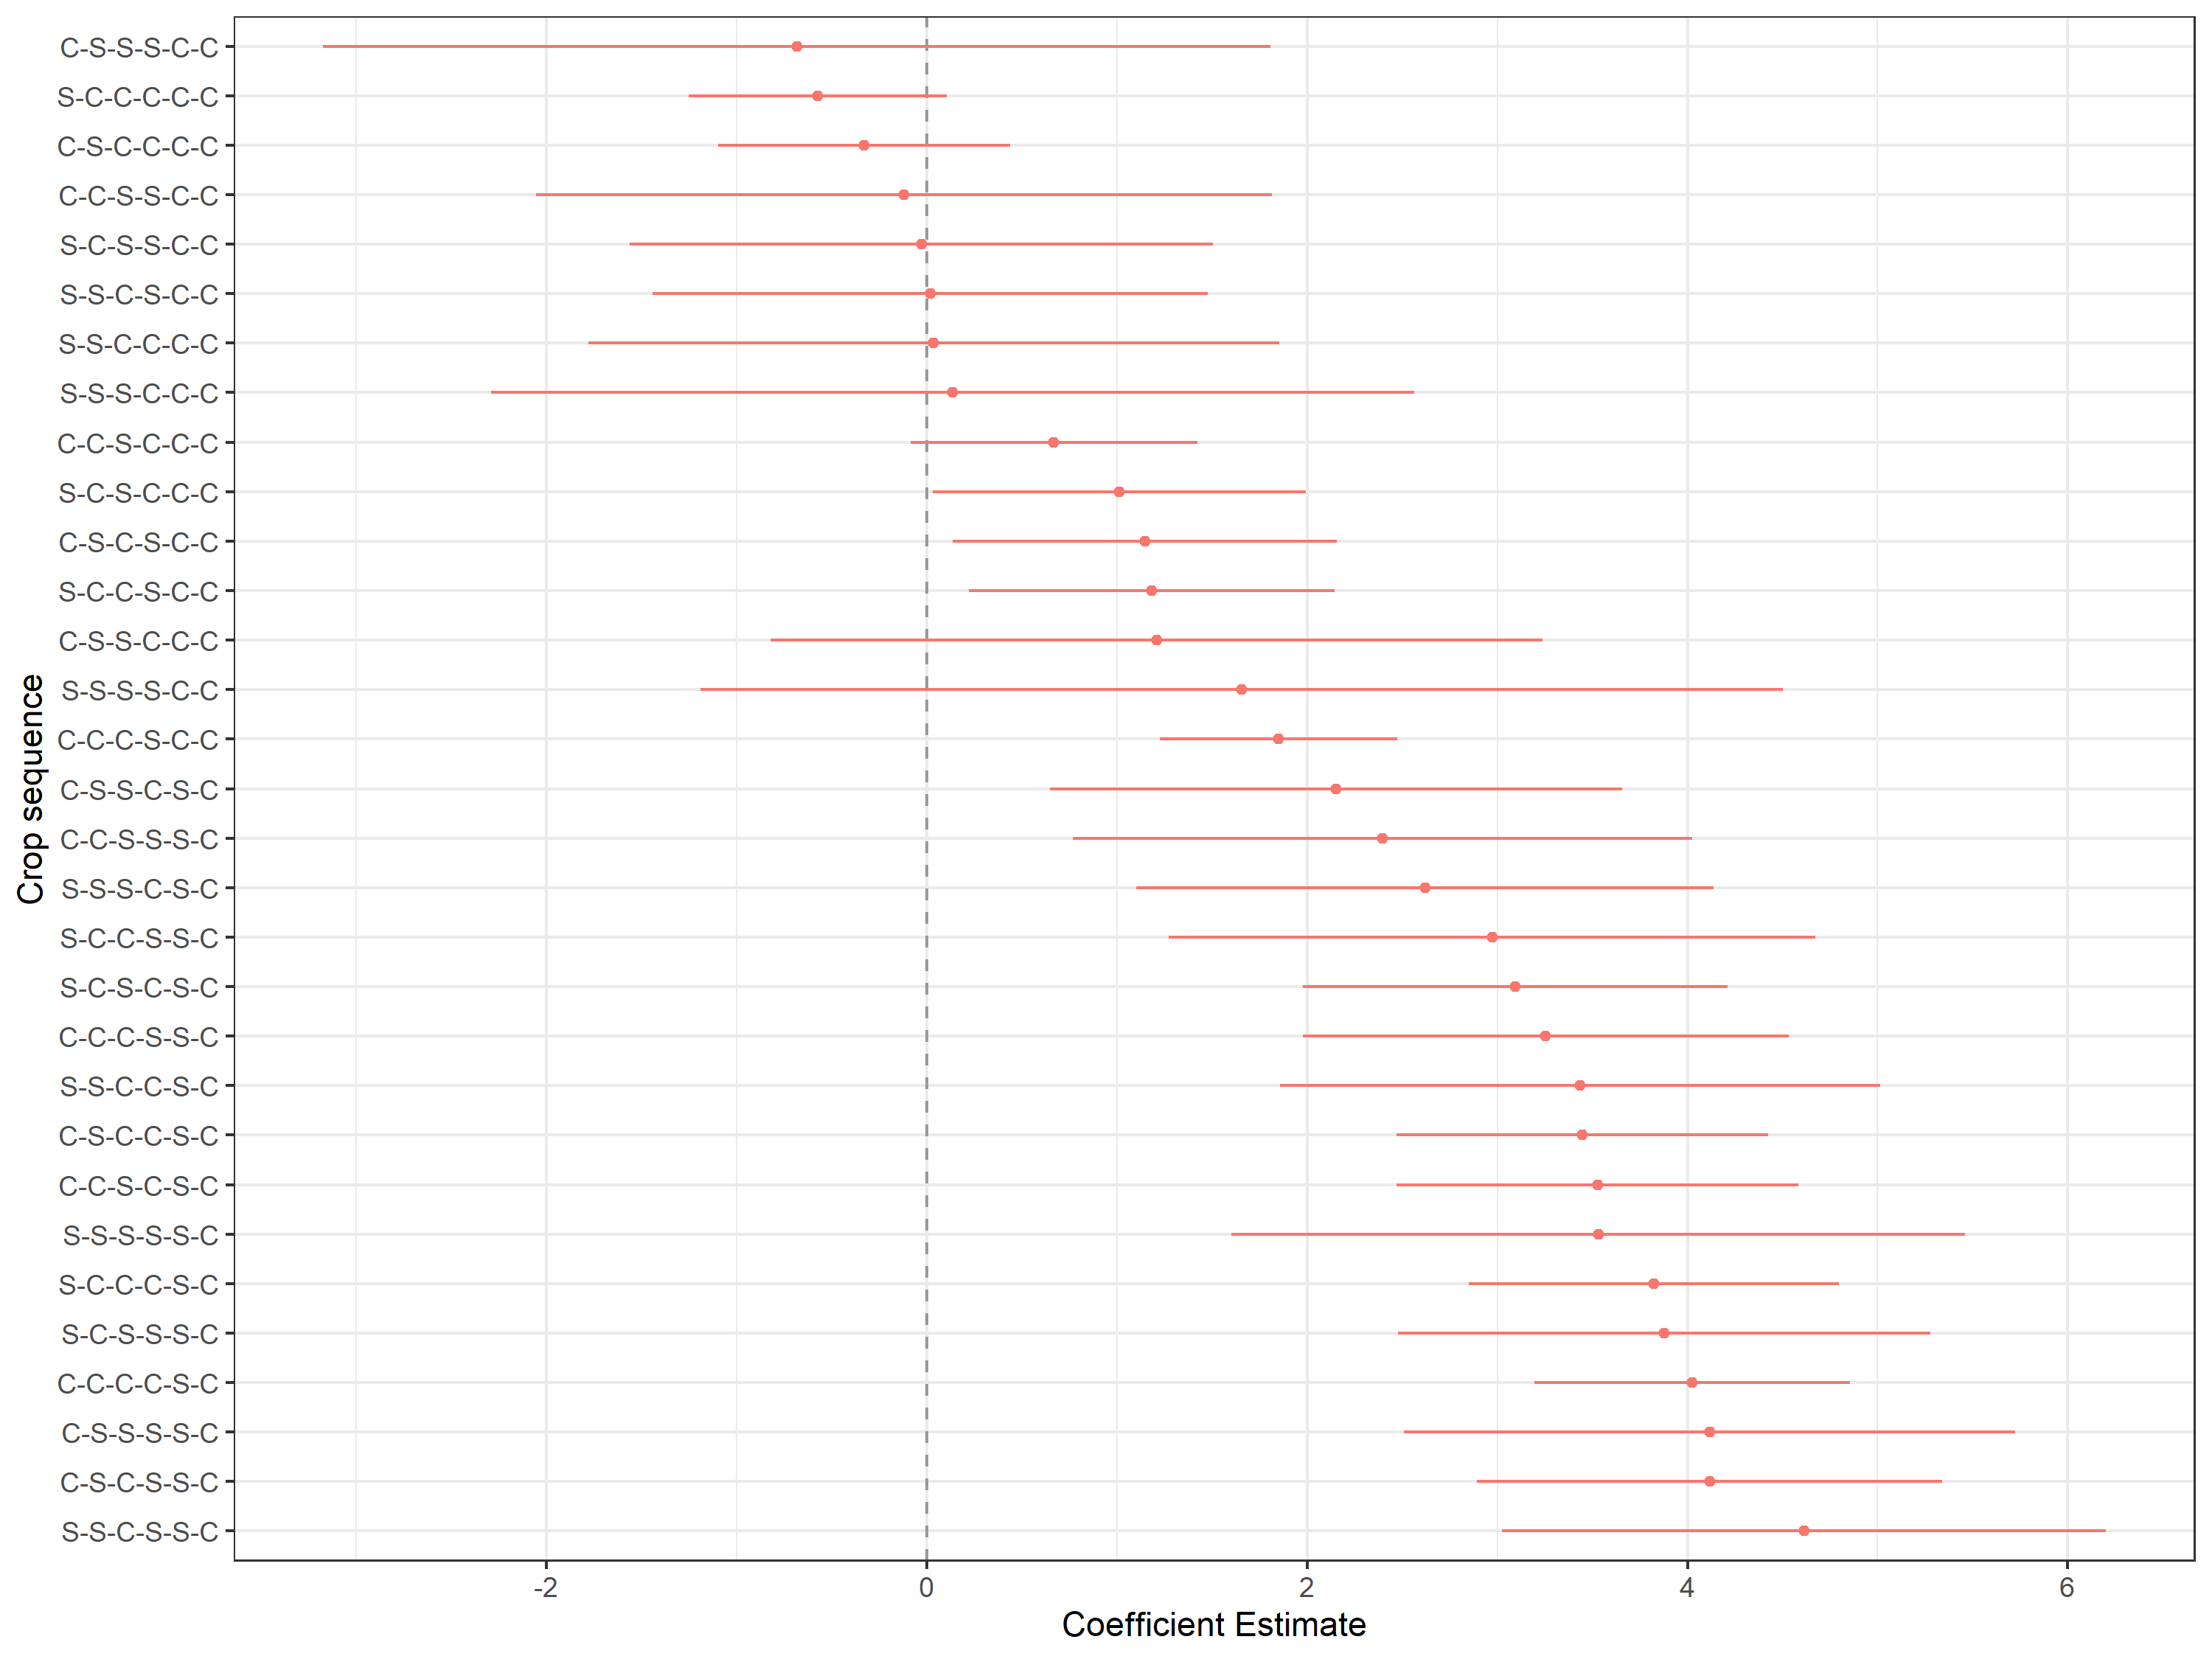
\includegraphics[scale = 0.55]{figures/corn_rot_plot.png}
    \caption{Response of corn yields to rotation sequences}
    \label{fig:corn_rot_plot}
    \end{figure}

    \begin{figure}[H]
    \centering
    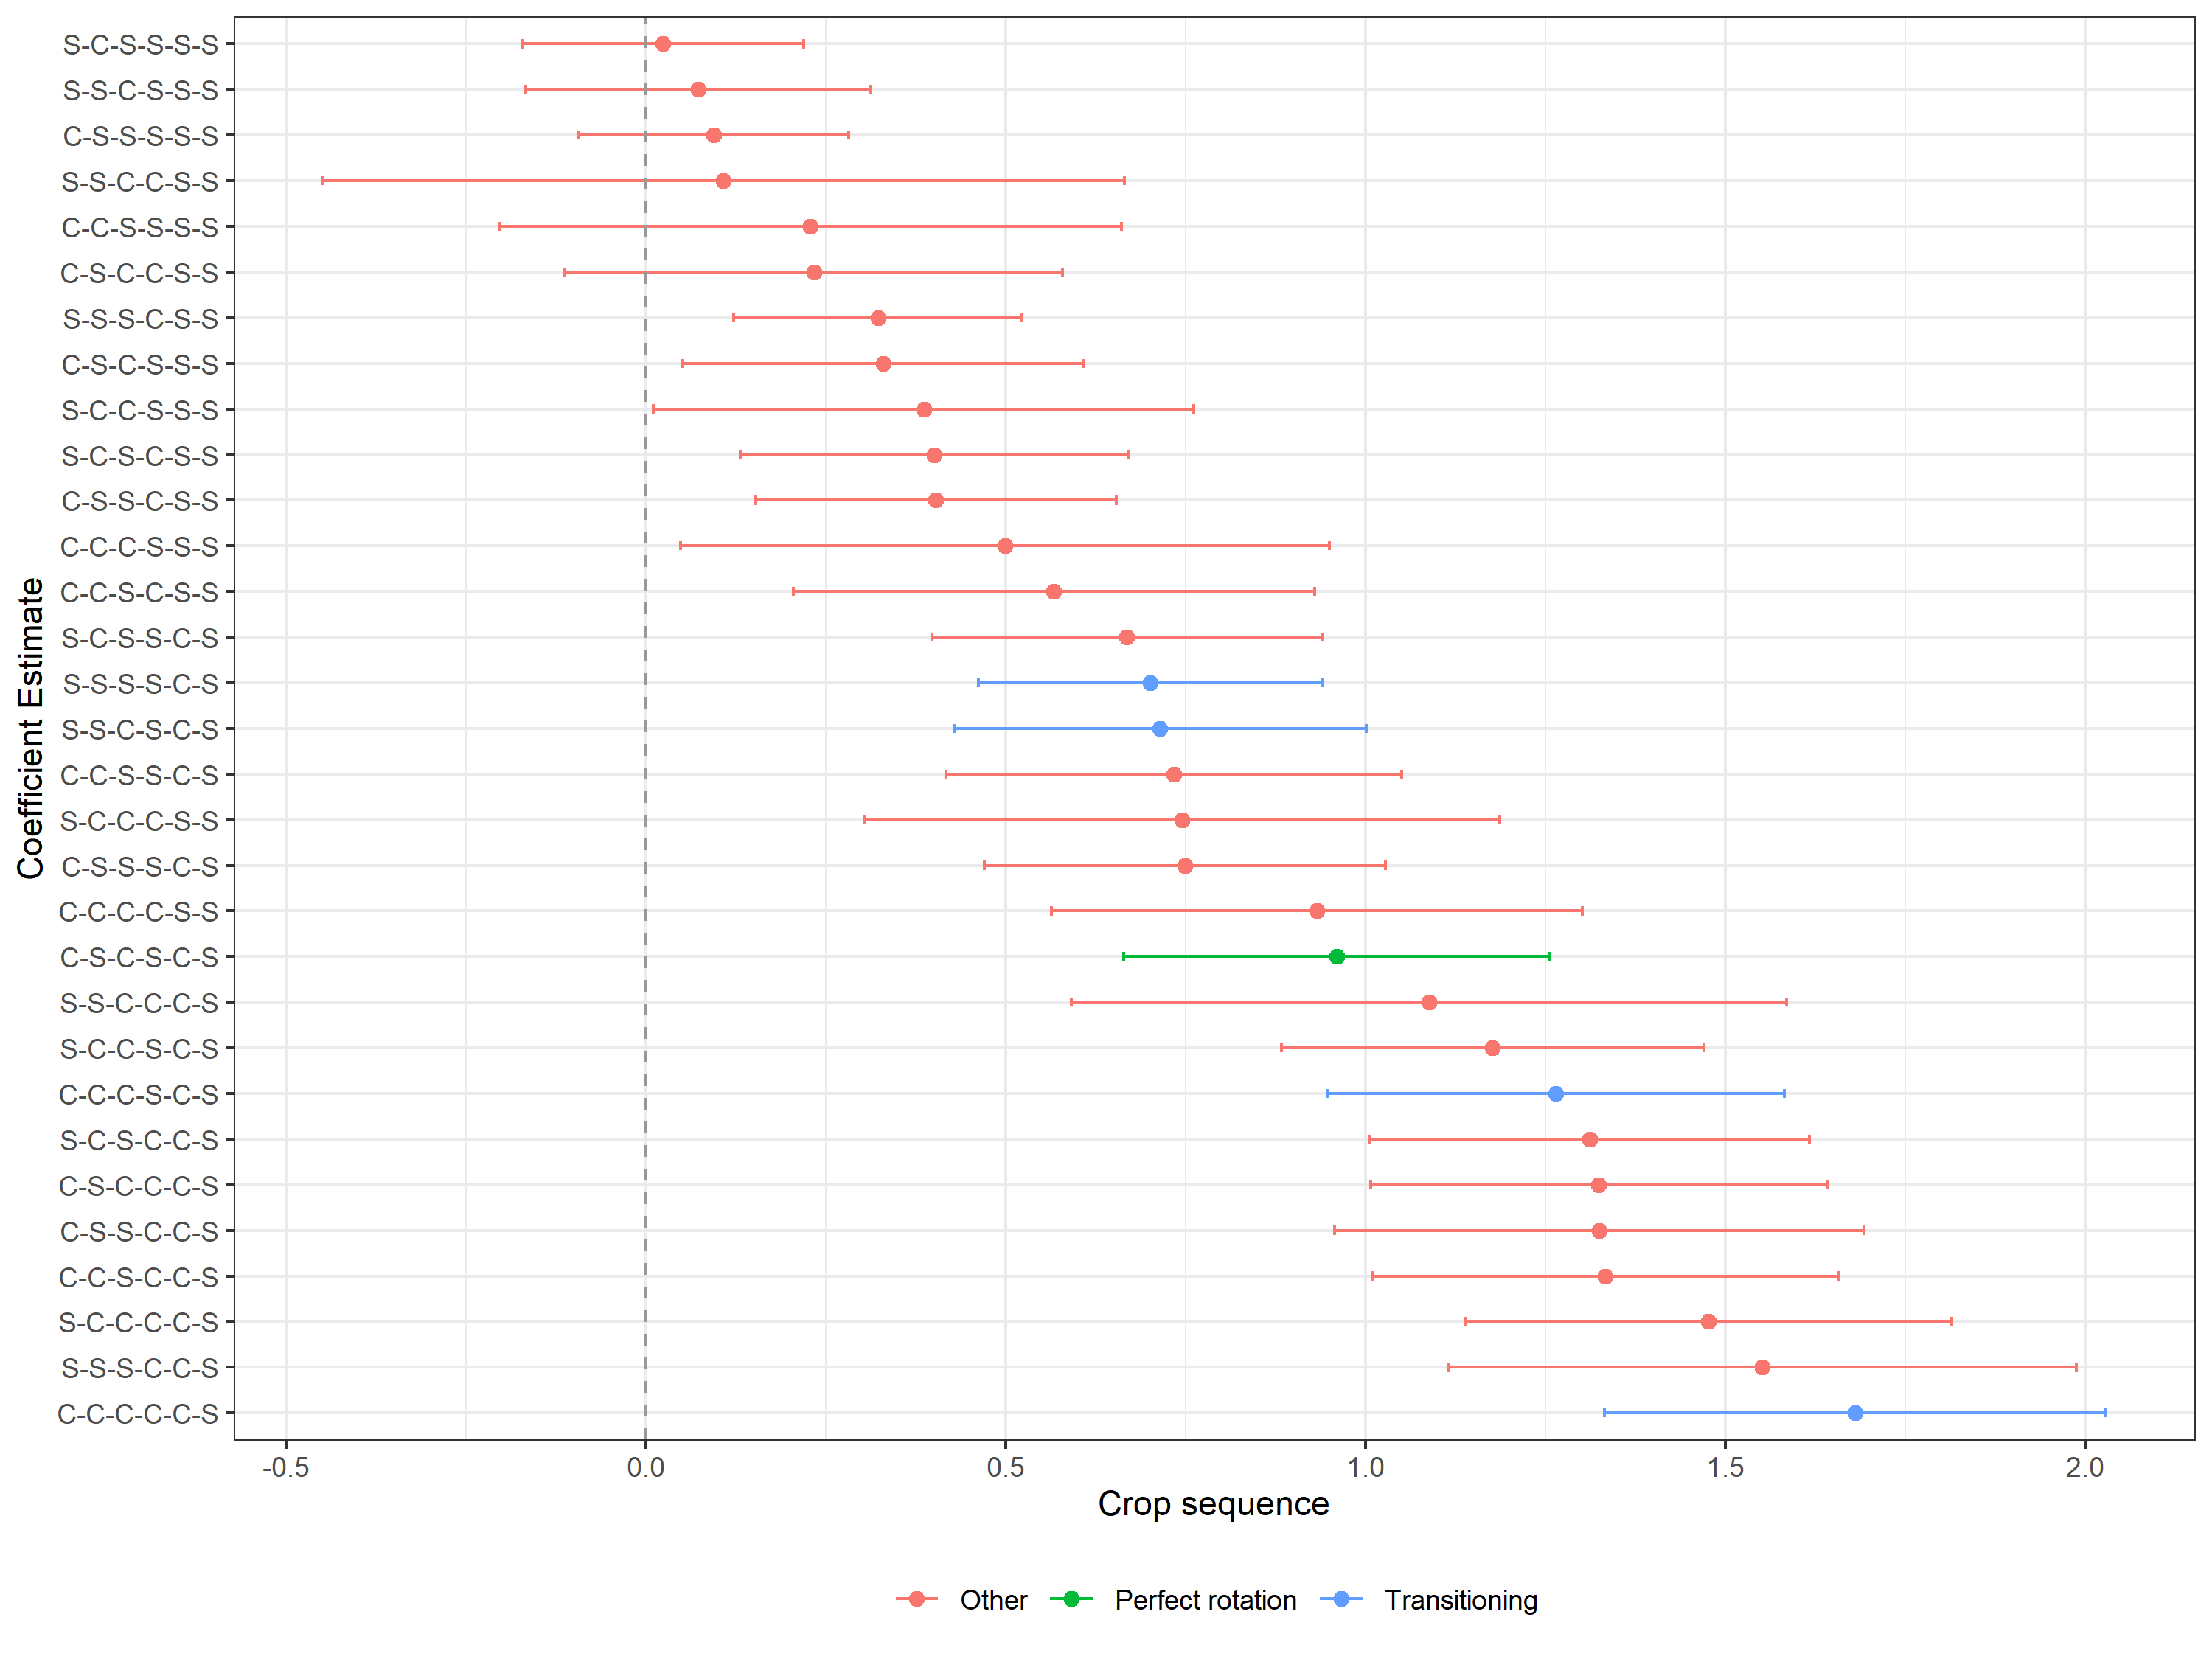
\includegraphics[scale = 0.55]{figures/soy_rot_plot.png}
    \caption{Response of soybean yields to rotation sequences}
    \label{fig:soy_rot_plot}
    \end{figure}

    \newpage
	\begin{figure}[H]
    \centering
    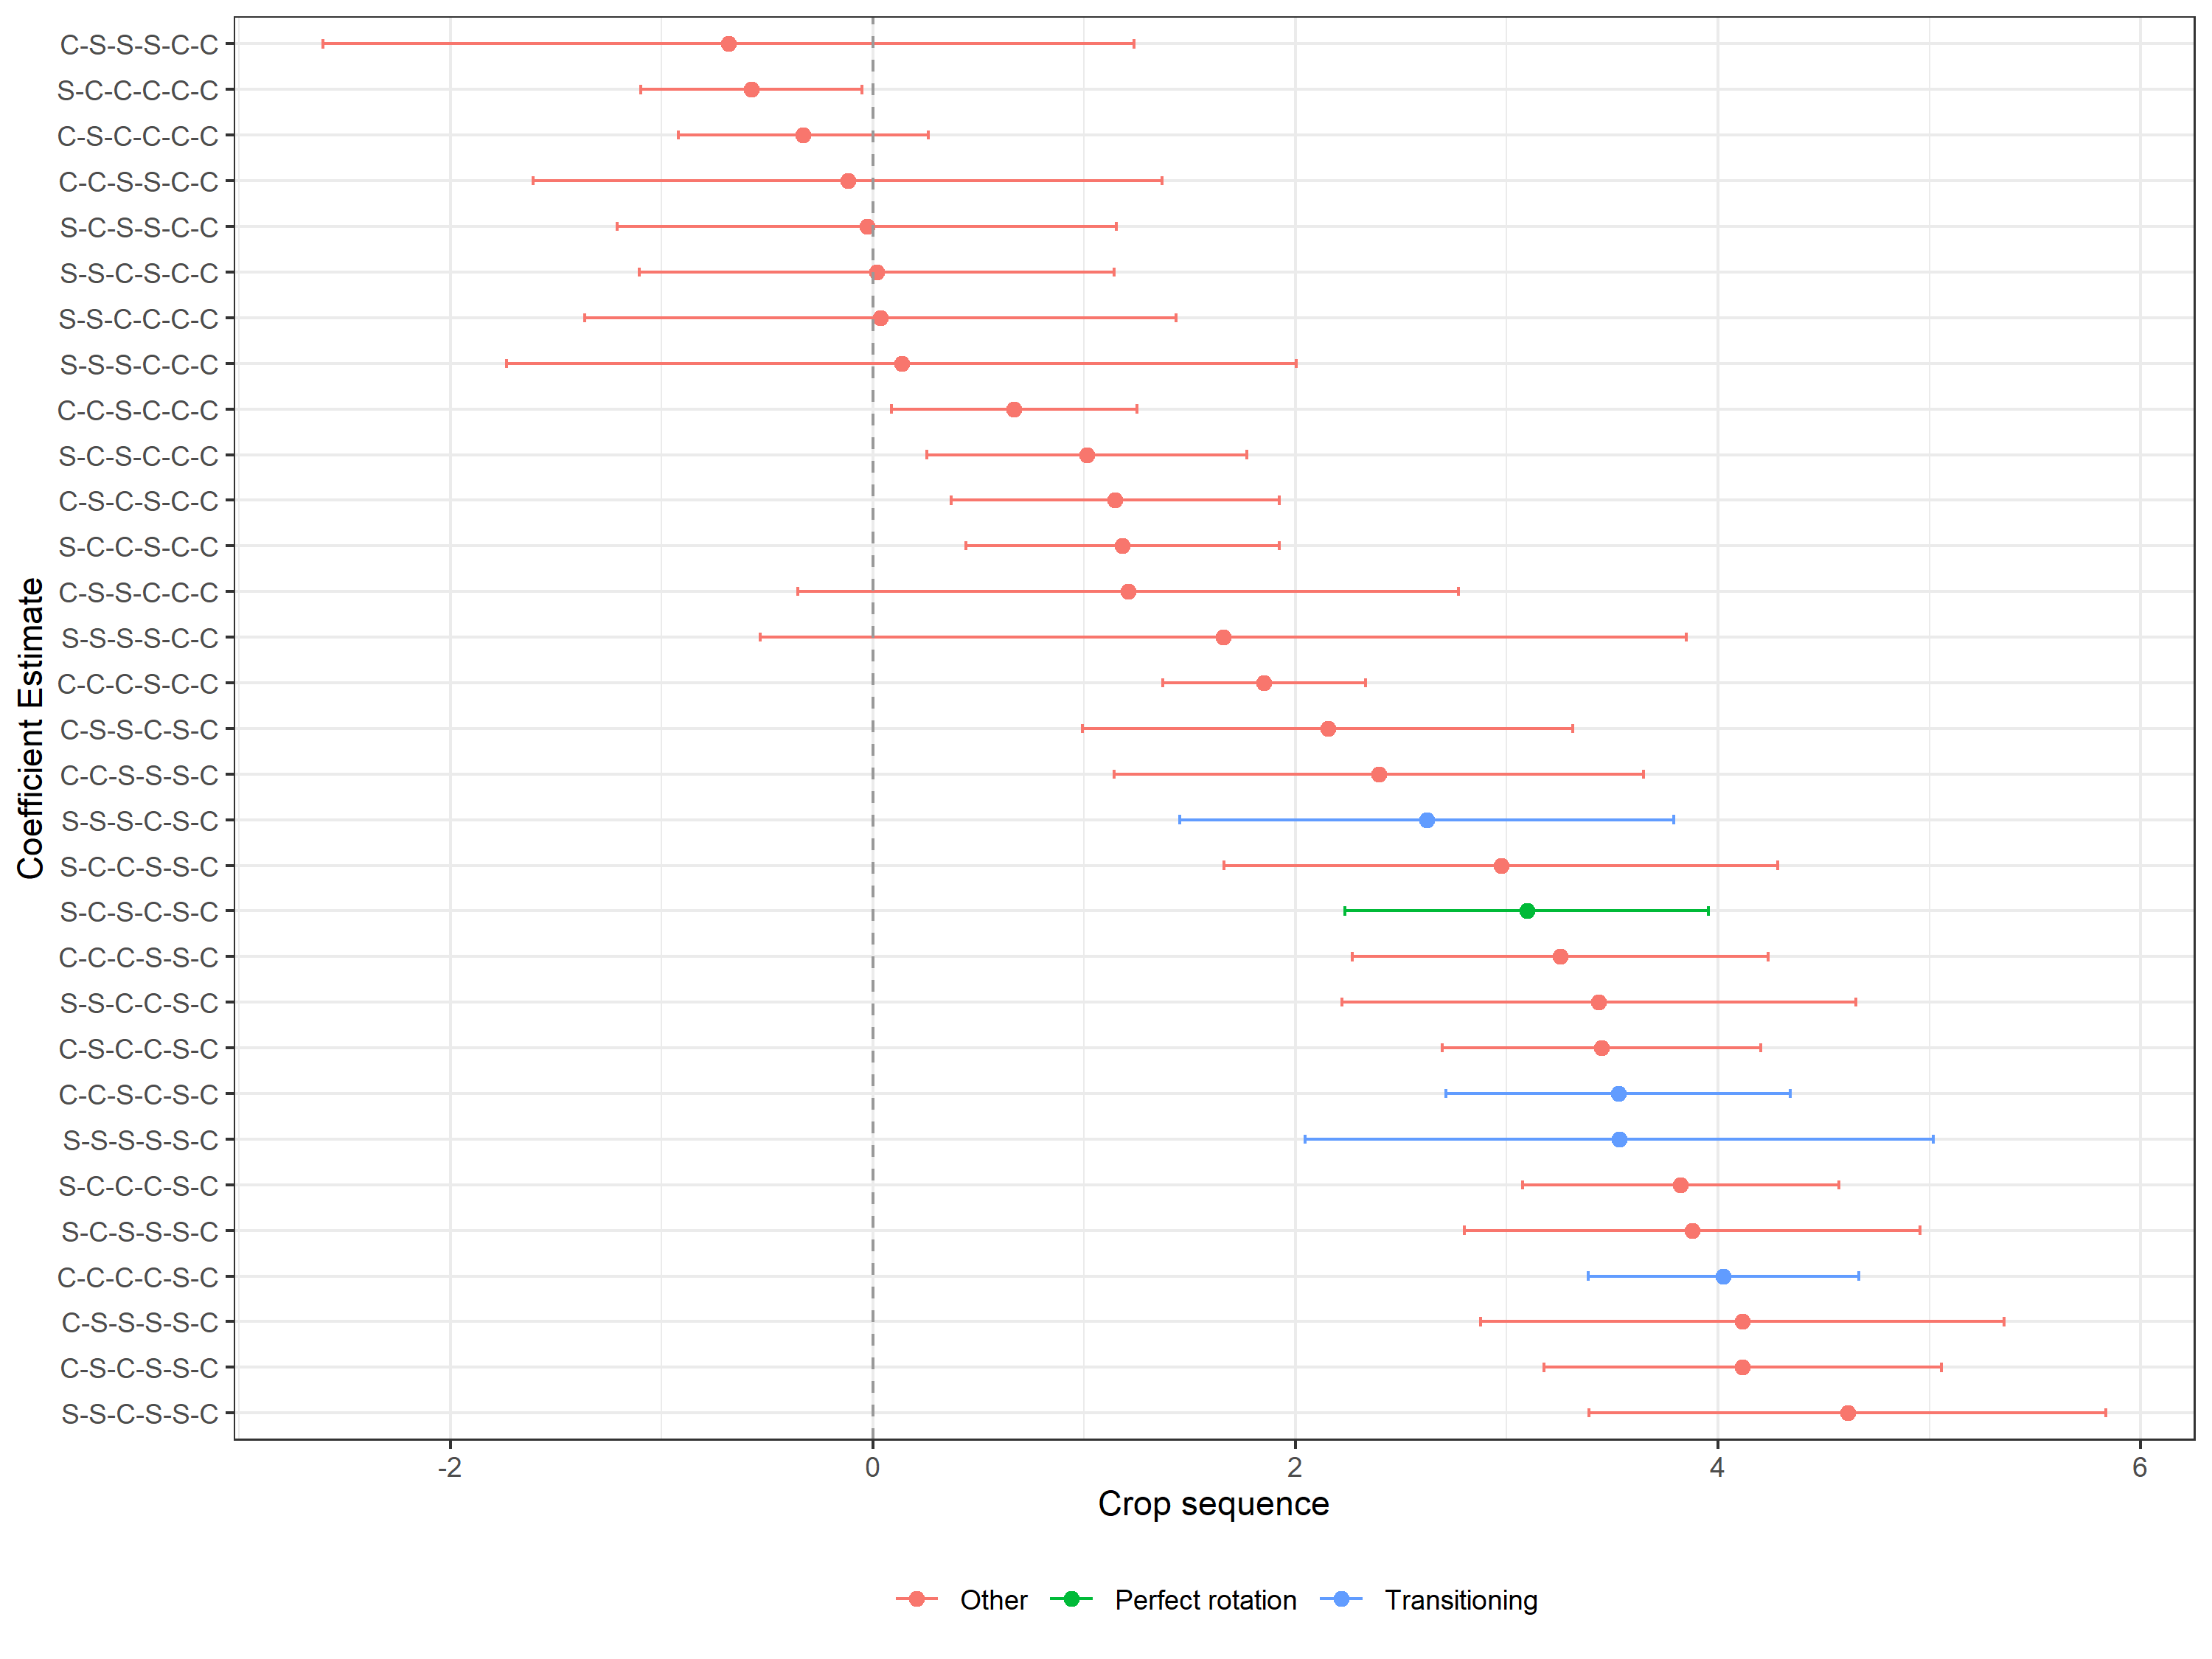
\includegraphics[scale = 0.55]{figures/corn_var_plot.png}
    \caption{Response of the standard deviation of corn yields to rotation sequences}
    \label{fig:corn_var_plot}
    \end{figure}

    \begin{figure}[H]
    \centering
    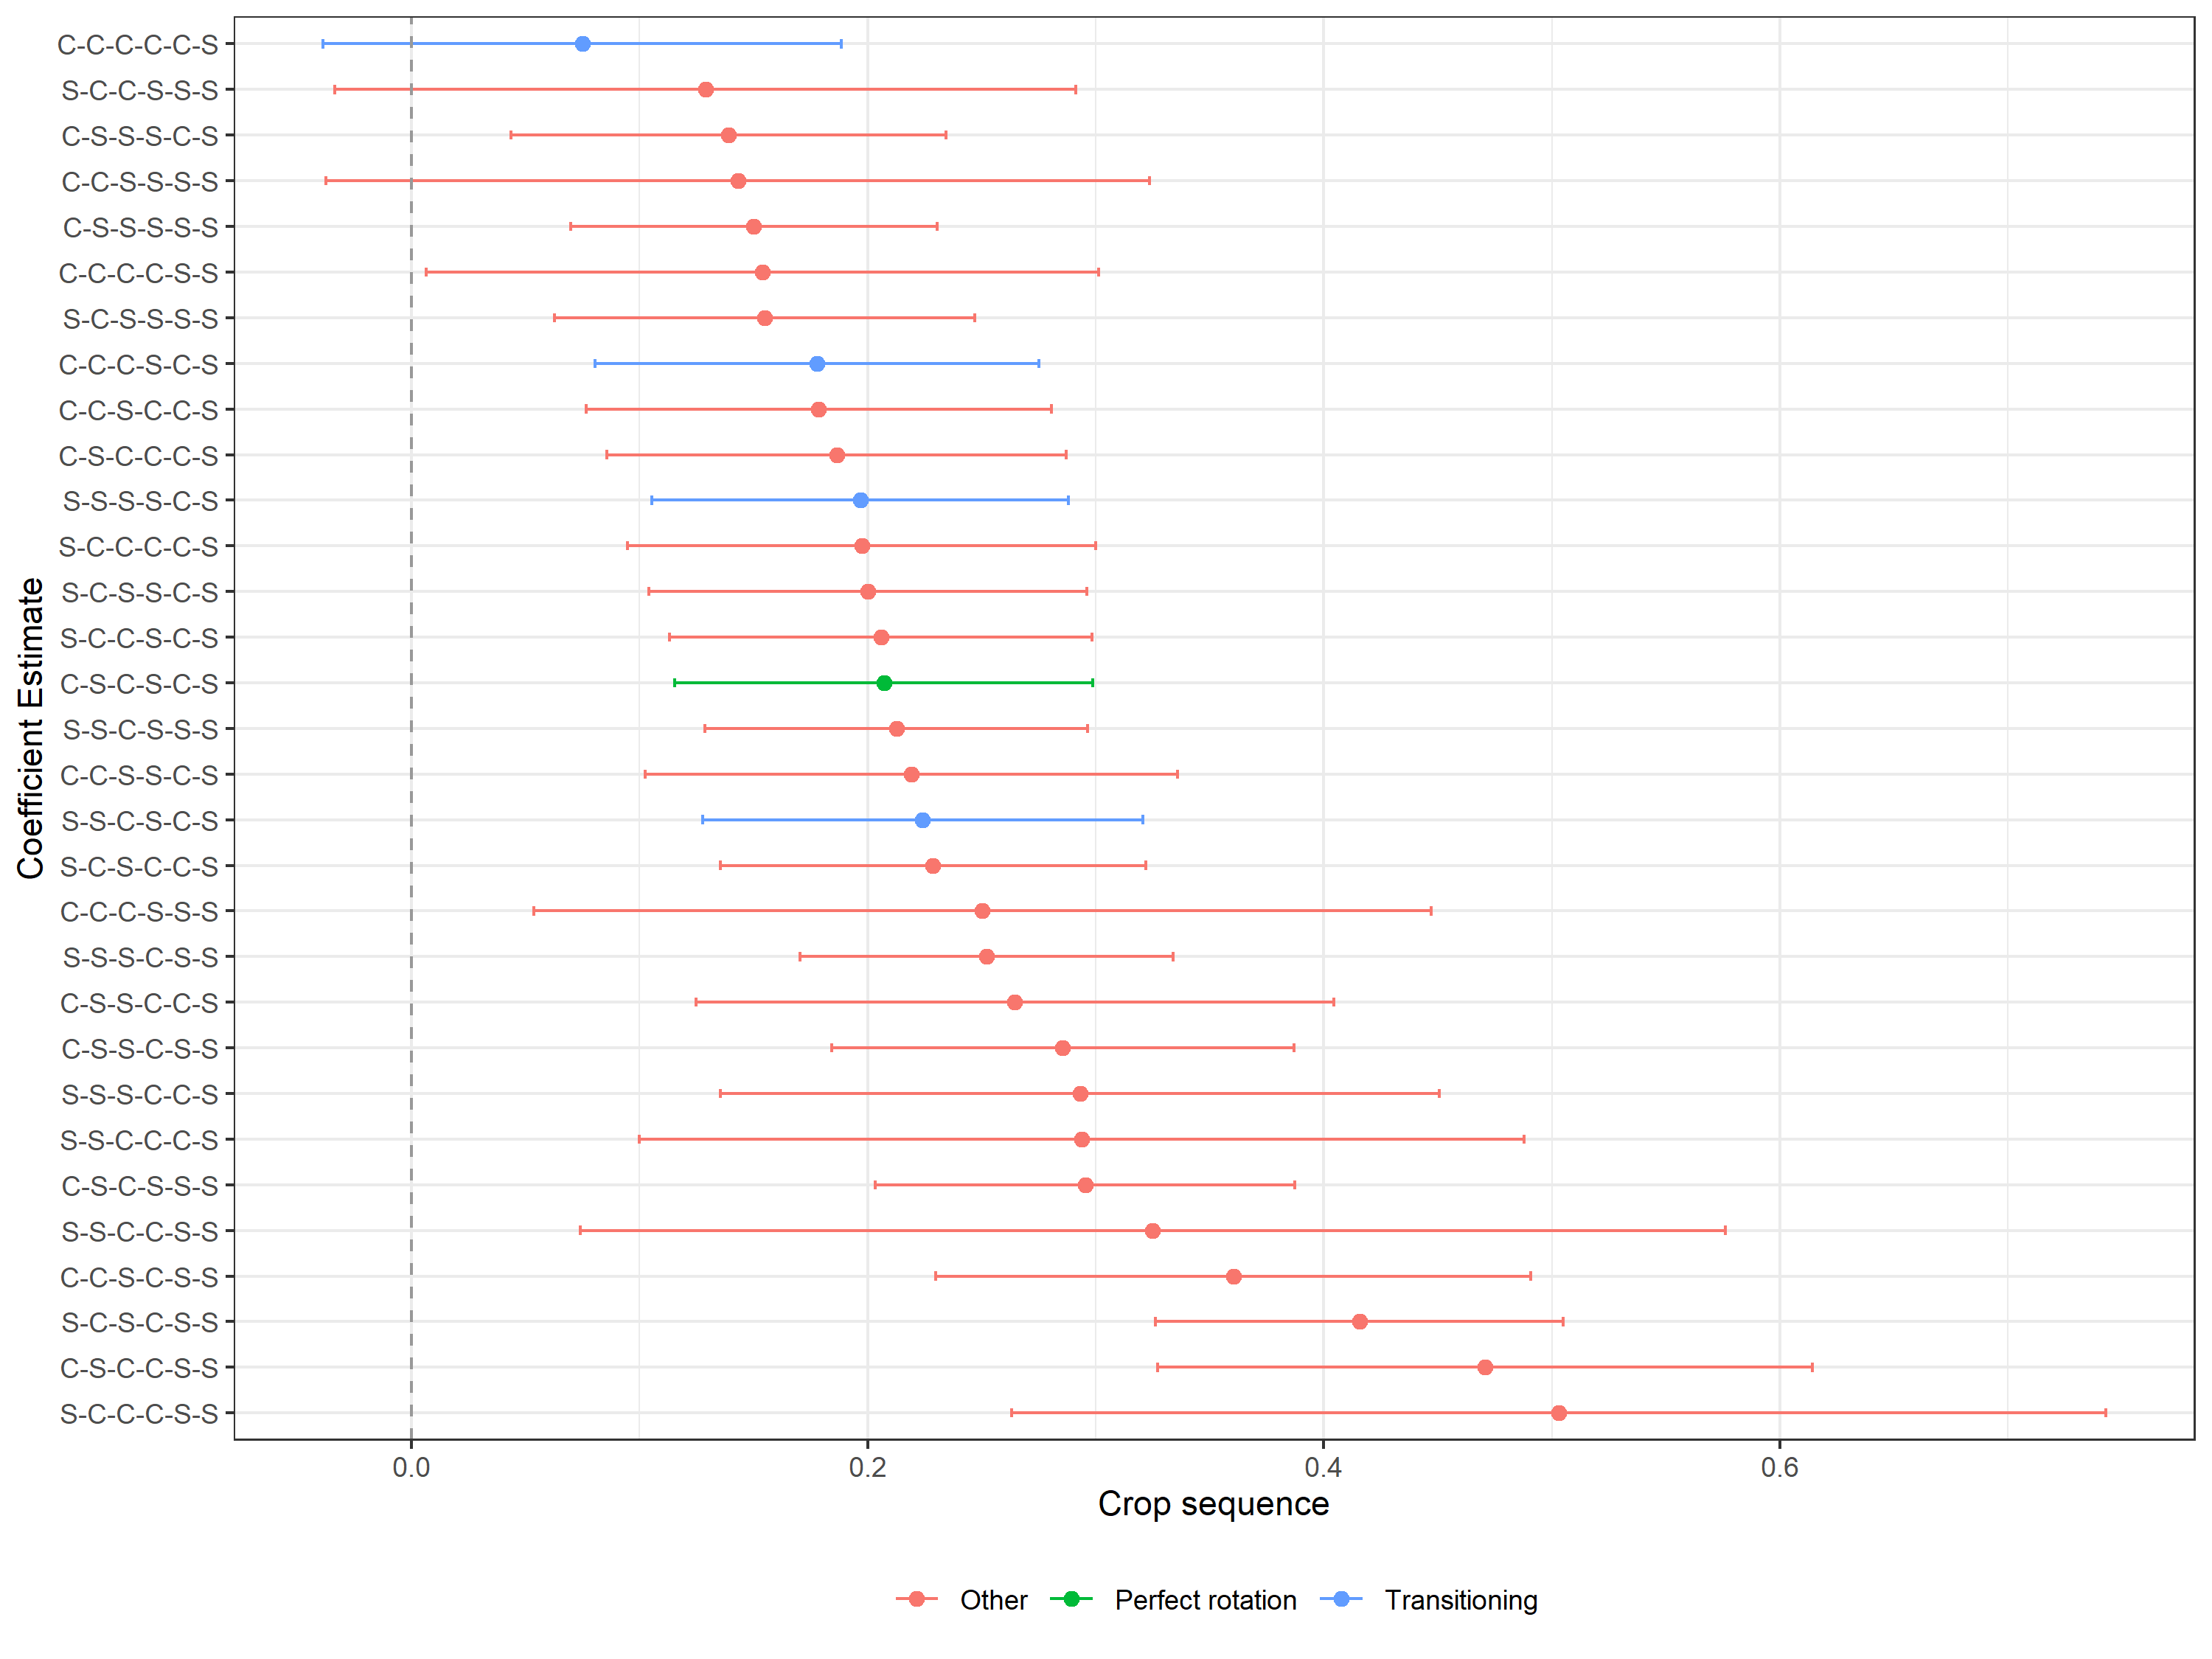
\includegraphics[scale = 0.55]{figures/soy_var_plot.png}
    \caption{Response of standard deviation of soybean yields to rotation sequences}
    \label{fig:soy_var_plot}
    \end{figure}
	
	\section{Results}
	\label{sec:results}
    Only a few sequences outperform corn monoculture in terms of higher mean/lower variance.
    
    Both SCYM and QDANN yield similar results. 
    
    Higher performing sequences have common elements:
    \begin{enumerate}
        \item A recent soy rotation (year 1 or 2).
        \item No consecutive soy years.
        \item Low impact of older crops (first three years).
        \item Perfect corn/soy rotation has positive but nonsignificant effects on yields, and reduces yield variance.
    \end{enumerate}

    We identified a set of rotation patterns that account for variations in first and second moments of corn yields.
    \begin{enumerate}
        \item Soy Lag: equal to the number of lagged periods a soy harvest was detected since the most recent year (e.g. if the latest soy harvest was the previous year, it takes a value equal to -1).
        \item Consecutive soy years: Dummy equal to 1 if a rotation pattern had two or more consecutive soy harvests.
        \item Soy gap: minimum number of years between two soy harvests (e.g. if two years of soy harvests occur, then the soy gap is 0).
        \item Number of soy harvests: how many times in the last seven years was a soy harvest detected?
    \end{enumerate}


    \newpage
    \begin{figure}[H]
    \centering
    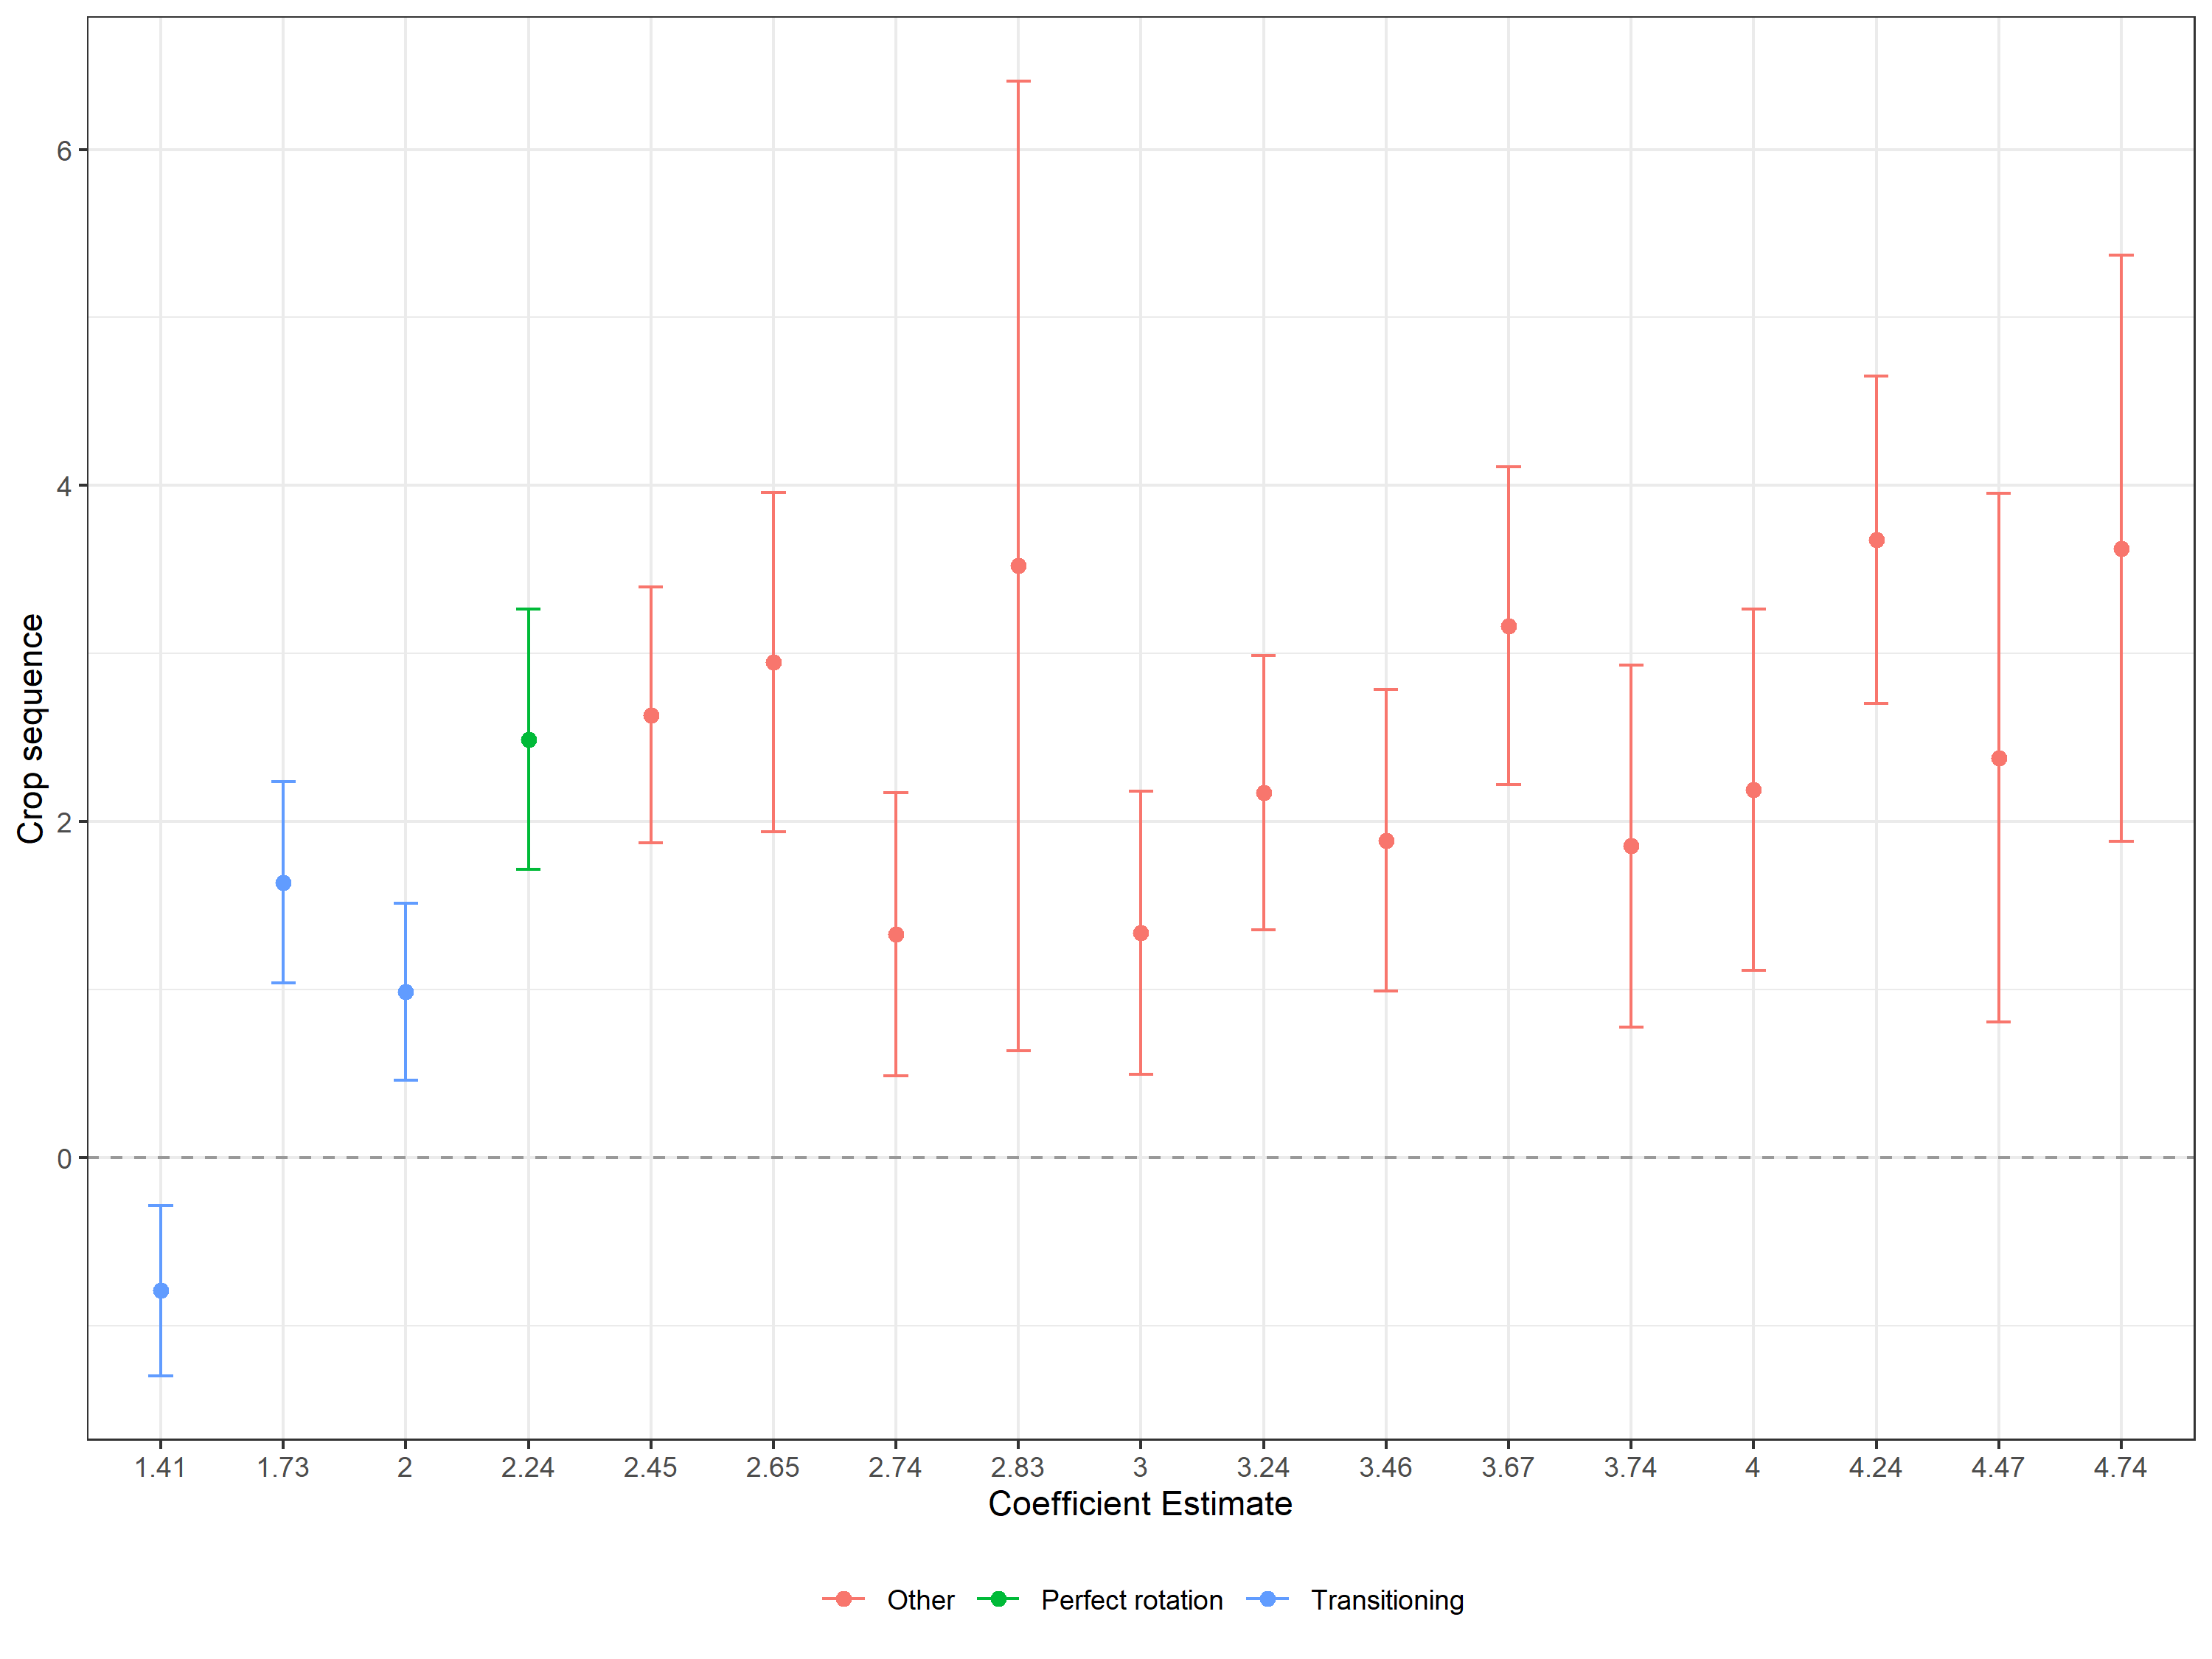
\includegraphics[scale = 0.55]{figures/corn_rci_plot.png}
    \caption{Changes on RCI and corn yields}
    \label{fig:corn_rci_plot} 
    \end{figure}

    \begin{figure}[H]
    \centering
    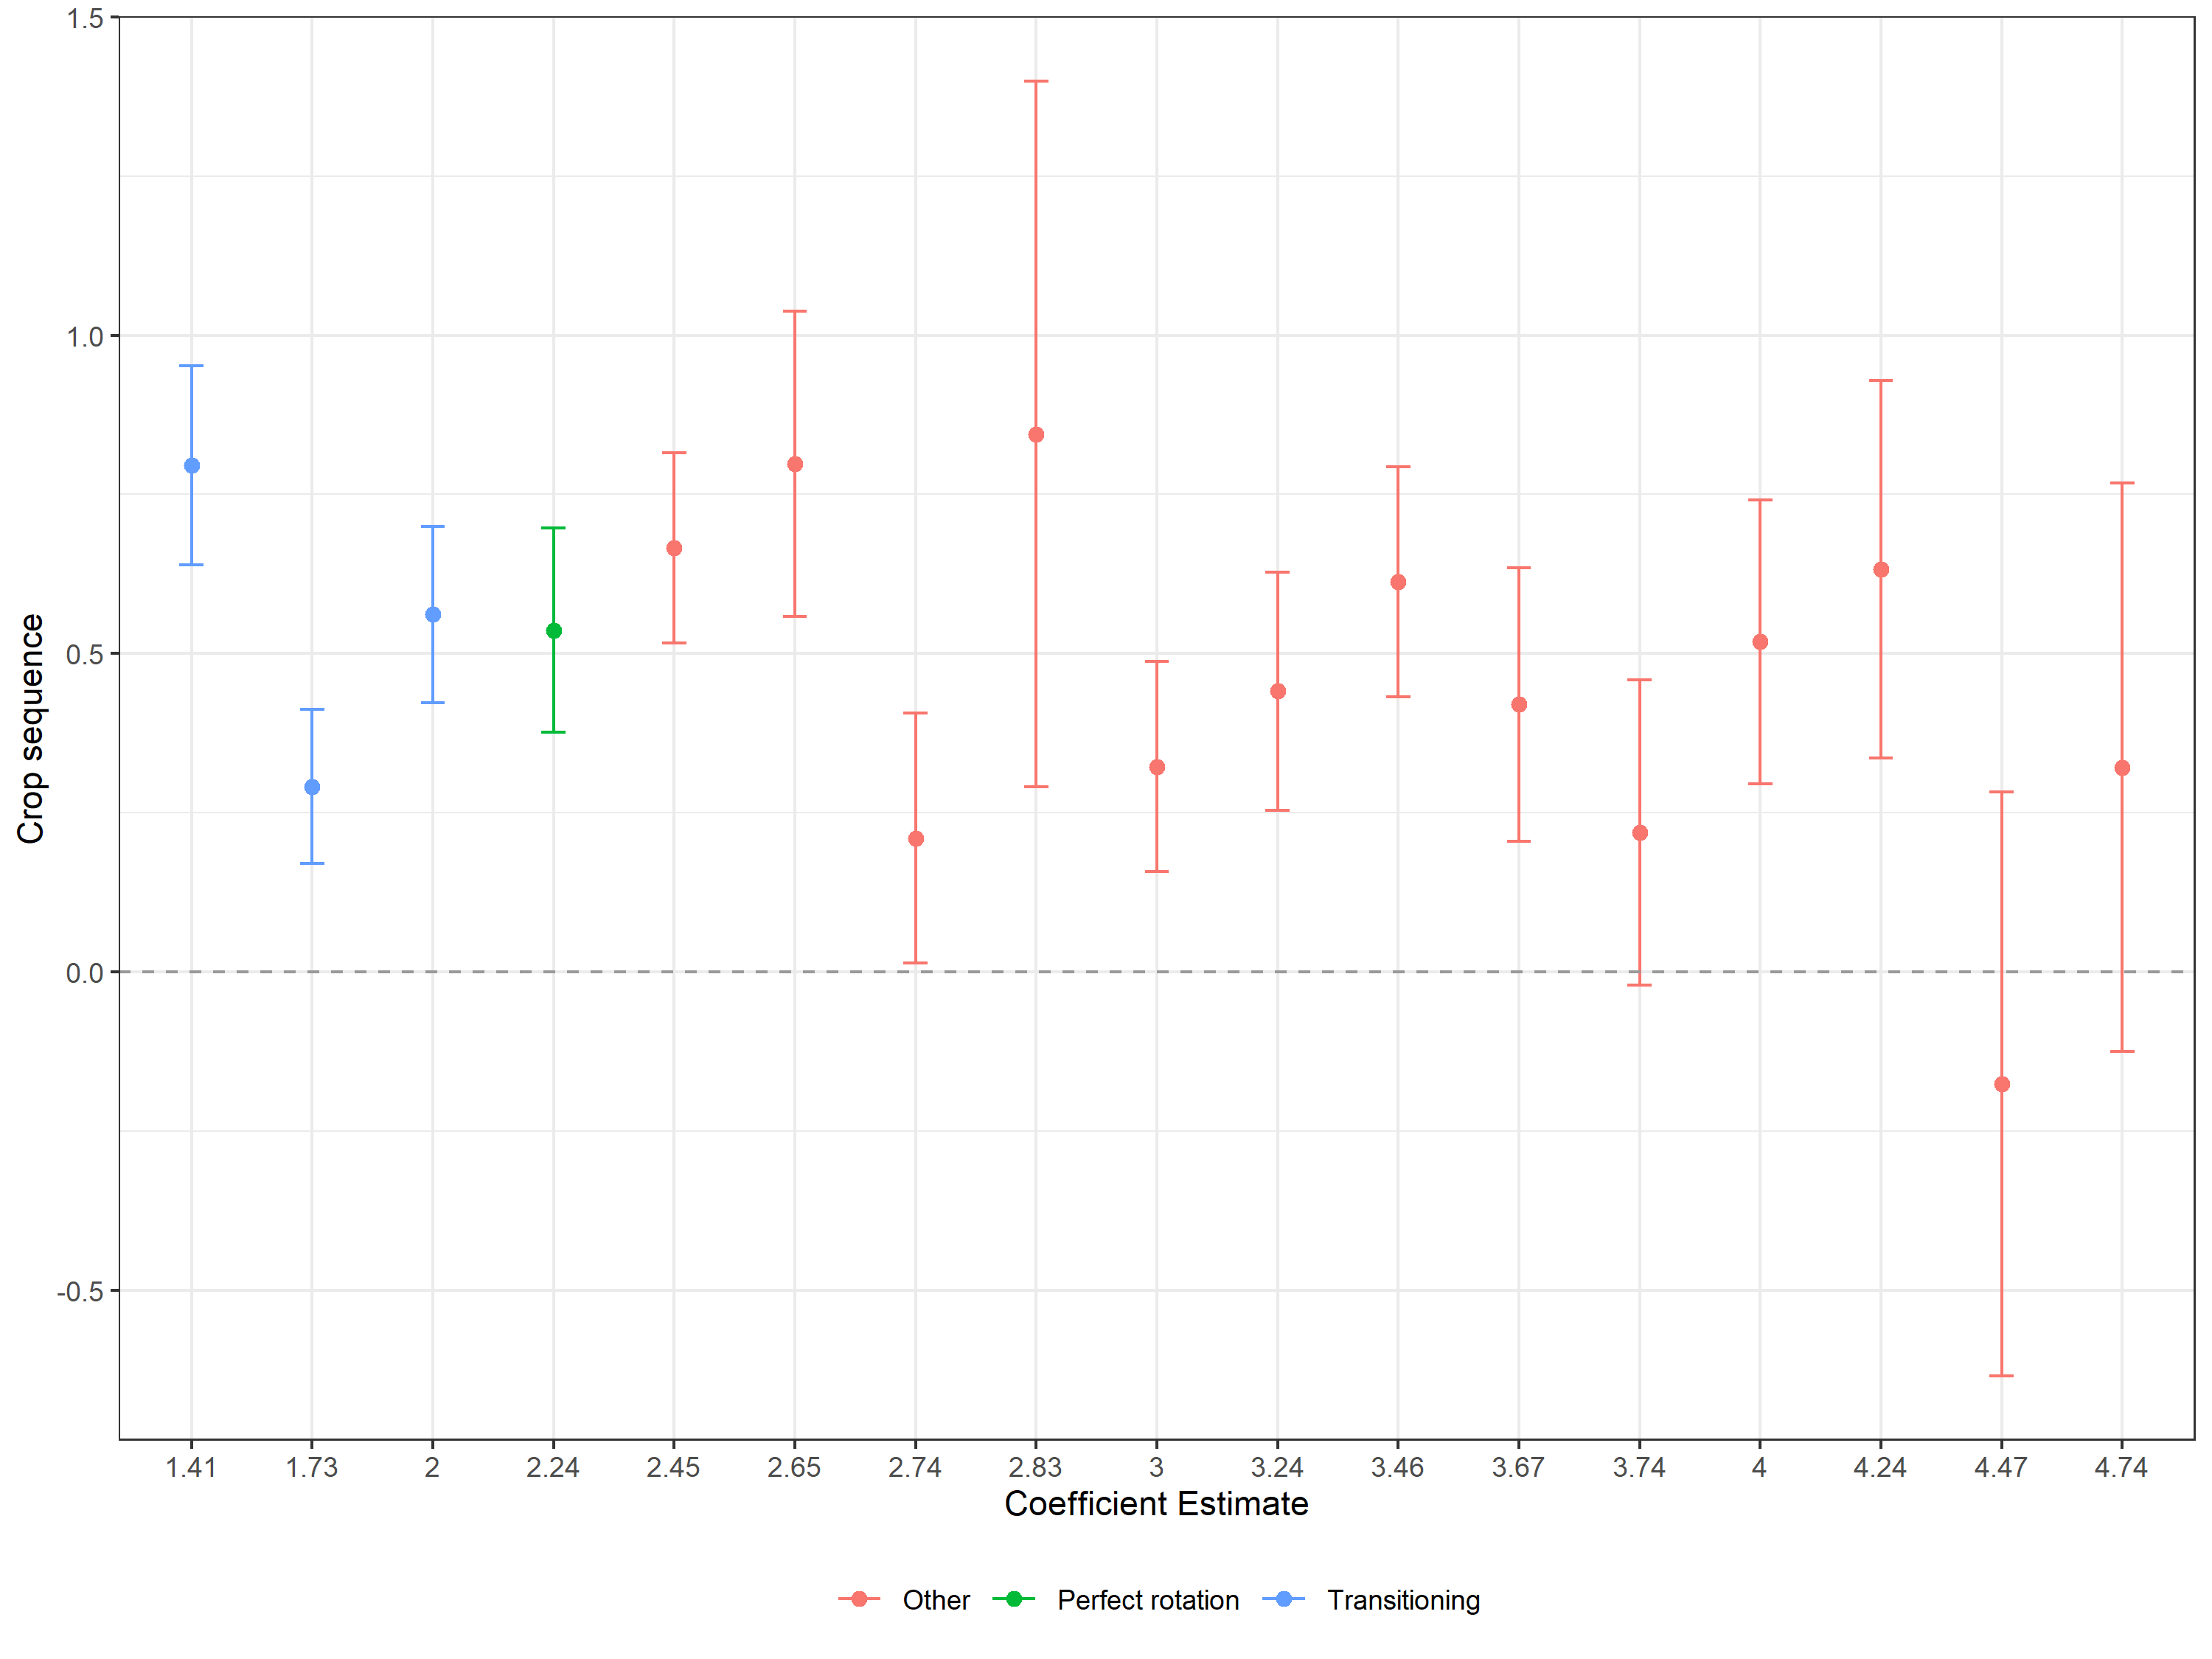
\includegraphics[scale = 0.55]{figures/soy_rci_plot.png}
    \caption{Changes in RCI and soybean yields}
    \label{fig:soy_rci_plot} 
    \end{figure}

    We model average yields as a linear FE model:
    \begin{equation*}
        y_{it}=Z\tau_{it}+W_{it}\beta_{it}+\lambda_{k}+\gamma_{t}+\varepsilon_{it}
    \end{equation*}
    
    Where: $Z = \left[late\_soy, soy\_cons,soy\_gap, nsoy\right]$
    
    
\begin{table}[htbp]
   \caption{\label{tab:fit1} Effect of rotation patterns on yields}
   \bigskip
   \centering
   \resizebox{0.85\textwidth}{!}{
   \begin{tabular}{lcccc}
      \toprule
      Variable                        & QDANN mean      & SCYM mean           & QDANN variance & SCYM variance \\   
      \midrule 
      Latest soy rotation             & 2.847$^{***}$   & 3.550$^{***}$       & -9.017$^{**}$  & 5.826\\   
                                      & (0.1663)        & (0.2167)            & (4.318)        & (6.843)\\   
      Soy gap                         & 0.3114$^{***}$  & 0.2466$^{***}$      & 2.611$^{**}$   & 6.177$^{***}$\\   
                                      & (0.0407)        & (0.0499)            & (1.181)        & (1.646)\\   
      Number of soy harvests          & -0.9760$^{***}$ & -1.080$^{***}$      & -11.17$^{***}$ & -32.93$^{***}$\\   
                                      & (0.1341)        & (0.1587)            & (3.198)        & (4.268)\\   
      Number of consecutive soy years & -4.671$^{***}$  & -4.171$^{***}$      & 79.18$^{***}$  & 133.9$^{***}$\\   
                                      & (0.2270)        & (0.2566)            & (5.649)        & (7.589)\\   
      Controls                        & Yes             & Yes                 & Yes            & Yes\\  
       \\
      Observations                    & 1,744,038       & 1,411,846           & 1,744,038      & 1,411,846\\  
      R$^2$                           & 0.57998         & 0.62967             & 0.05231        & 0.03429\\  
      Within R$^2$                    & 0.20564         & 0.17989             & 0.01483        & 0.00676\\  
       \\
      year fixed effects              & $\checkmark$    & $\checkmark$        & $\checkmark$   & $\checkmark$\\   
      fips fixed effects      & $\checkmark$    & $\checkmark$        & $\checkmark$   & $\checkmark$\\   
      \bottomrule
   \end{tabular}}
\end{table}




   % All four variables can be used to construct a \textbf{rotation score}:
   % \begin{equation*}
    %score_{it}=\hat{\beta}_{1}late\_soy_{it}+\hat{\beta}_{2}soy\_cons_{it}+\hat{\beta}_{3}soy\_gap_{it}+\hat{\beta}_{4}nsoy_{it}
    %\end{equation*}
    
    %This score summarizes the information from the four variables and allows us to classify the 64 rotation patterns into a smaller set of values.
    
    %Score values for corn monoculture are 0, and for perfect rotation, 2.59.
    
    %We predict yields based on rotation score and summarize our findings.

    %\begin{figure}[H]
    %\centering
    %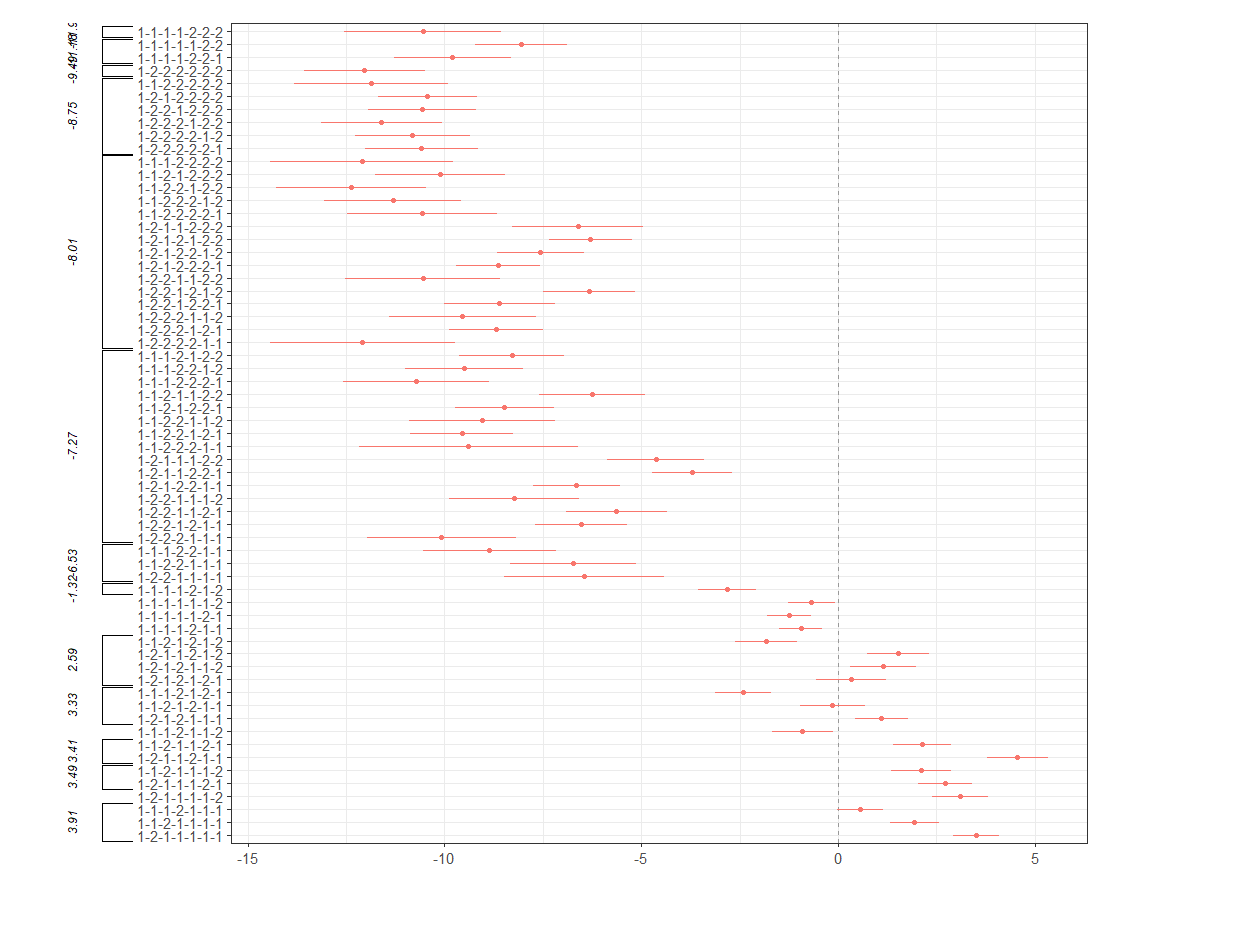
\includegraphics[scale = 0.75]{figures/rot_score.png}
    %\caption{Response of yields to rotation sequences}
    %\label{fig:rot_score} 
    %\end{figure}

    %\begin{figure}[H]
    %\centering
    %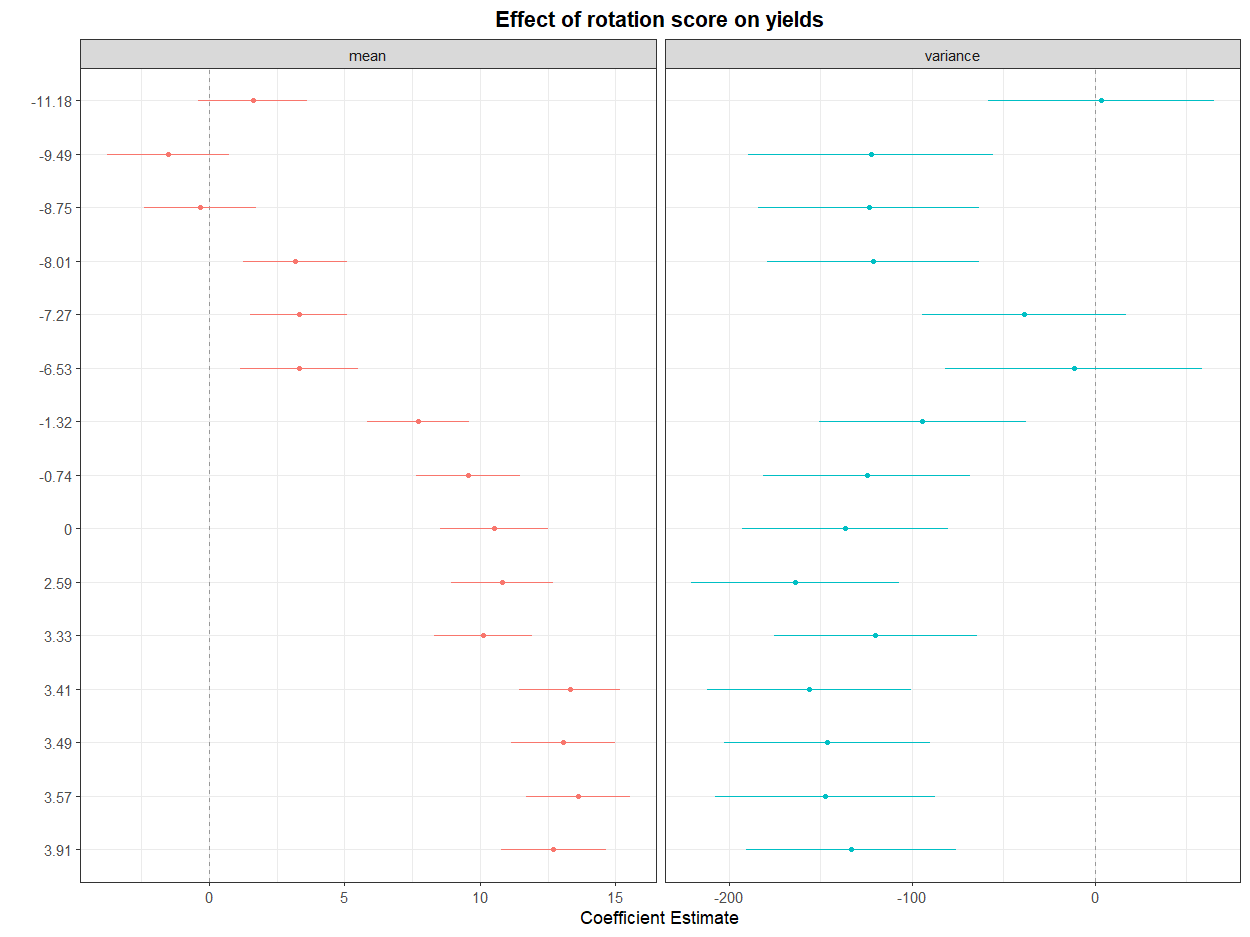
\includegraphics[scale = 0.65]{figures/mean_var_score.png}
    %\caption{Response of yields to score values}
    %\label{fig:rot_score} 
    %\end{figure}
    
	\newpage
	\bibliography{bibliography.bib}

    \newpage
	\appendix
	
	\section{Appendix 1 \ref{sec:appendix}}
    \subsection{Rotation patterns and yield coefficients}
	
\begin{table}[H]
   \caption{\label{tab:corn_rot} Rotation patterns and corn yields}
   \bigskip
   \centering
   \scriptsize
   \renewcommand*{\arraystretch}{0.8}
   \begin{tabular}{lcc}
      \toprule
       & \multicolumn{2}{c}{corn\_yield}\\
                                      & No controls              & With controls \\   
                                      & (1)                      & (2)\\  
      \midrule 
      W-C-C-S-W-C                     & 8.329$^{***}$ (1.537) [p<0.001]    & 7.630$^{***}$ (1.496) [p<0.001]\\   
      C-S-C-W-S-C                     & 8.170$^{***}$ (1.492) [p<0.001]    & 6.311$^{***}$ (1.368) [p<0.001]\\   
      S-S-C-S-S-C                     & 6.861$^{***}$ (0.5615) [p<0.001]   & 5.938$^{***}$ (0.5157) [p<0.001]\\   
      C-C-C-S-W-C                     & 6.826$^{***}$ (0.6815) [p<0.001]   & 5.810$^{***}$ (0.6512) [p<0.001]\\   
      S-C-S-W-S-C                     & 6.292$^{***}$ (0.6945) [p<0.001]   & 5.772$^{***}$ (0.6868) [p<0.001]\\   
      C-S-C-S-S-C                     & 5.430$^{***}$ (0.4847) [p<0.001]   & 4.824$^{***}$ (0.4312) [p<0.001]\\   
      S-S-S-S-S-C                     & 5.061$^{***}$ (0.6902) [p<0.001]   & 4.655$^{***}$ (0.5542) [p<0.001]\\   
      S-C-S-S-S-C                     & 5.270$^{***}$ (0.5453) [p<0.001]   & 4.609$^{***}$ (0.4616) [p<0.001]\\   
      C-C-C-C-S-C                     & 4.628$^{***}$ (0.3541) [p<0.001]   & 4.411$^{***}$ (0.3639) [p<0.001]\\   
      S-S-C-C-S-C                     & 5.004$^{***}$ (0.5438) [p<0.001]   & 4.308$^{***}$ (0.5122) [p<0.001]\\   
      C-S-S-S-S-C                     & 4.305$^{***}$ (0.6044) [p<0.001]   & 4.284$^{***}$ (0.5434) [p<0.001]\\   
      S-C-C-C-S-C                     & 4.696$^{***}$ (0.3683) [p<0.001]   & 4.230$^{***}$ (0.3499) [p<0.001]\\   
      S-C-C-S-W-C                     & 5.012$^{***}$ (0.7216) [p<0.001]   & 4.121$^{***}$ (0.6876) [p<0.001]\\   
      C-S-C-C-S-C                     & 4.494$^{***}$ (0.3984) [p<0.001]   & 4.089$^{***}$ (0.3658) [p<0.001]\\   
      C-C-S-C-S-C                     & 4.286$^{***}$ (0.4121) [p<0.001]   & 4.071$^{***}$ (0.3928) [p<0.001]\\   
      C-C-C-S-S-C                     & 3.602$^{***}$ (0.5559) [p<0.001]   & 3.746$^{***}$ (0.5121) [p<0.001]\\   
      S-C-S-C-S-C                     & 4.195$^{***}$ (0.4310) [p<0.001]   & 3.632$^{***}$ (0.3953) [p<0.001]\\   
      S-C-C-S-S-C                     & 3.943$^{***}$ (0.6356) [p<0.001]   & 3.287$^{***}$ (0.5725) [p<0.001]\\   
      S-S-S-C-S-C                     & 3.650$^{***}$ (0.5843) [p<0.001]   & 3.250$^{***}$ (0.5012) [p<0.001]\\   
      C-C-C-S-C-C                     & 2.463$^{***}$ (0.2341) [p<0.001]   & 2.105$^{***}$ (0.2482) [p<0.001]\\   
      C-S-C-S-C-C                     & 1.436$^{***}$ (0.3704) [p<0.001]   & 1.028$^{***}$ (0.3617) [p=0.005]\\   
      S-C-S-S-C-C                     & 1.214$^{**}$ (0.5779) [p=0.038]    & 0.6850 (0.5368) [p=0.205]\\   
      C-C-S-C-C-C                     & 0.9810$^{***}$ (0.2932) [p=0.001]  & 0.6844$^{**}$ (0.2820) [p=0.017]\\   
      S-C-S-C-C-C                     & 0.9022$^{***}$ (0.3191) [p=0.006]  & 0.4936 (0.3144) [p=0.119]\\   
      S-S-C-S-C-C                     & 0.0523 (0.6005) [p=0.931]          & -0.6638 (0.5569) [p=0.236]\\   
      C-S-C-C-C-C                     & -0.6166$^{**}$ (0.2826) [p=0.031]  & -0.7695$^{***}$ (0.2520) [p=0.003]\\   
      S-C-C-C-C-C                     & -0.7831$^{***}$ (0.2424) [p=0.002] & -1.076$^{***}$ (0.2311) [p<0.001]\\   
      S-S-C-C-C-C                     & -1.096 (0.7090) [p=0.125]          & -1.326$^{**}$ (0.6373) [p=0.040]\\   
       \\
      Observations                    & 1,796,806                & 1,796,806\\  
      R$^2$                           & 0.81623                  & 0.84354\\  
      Within R$^2$                    & 0.00690                  & 0.15452\\  
      Controls                        & No                       & Yes\\  
       \\
      tile\_field\_ID fixed effects   & $\checkmark$             & $\checkmark$\\   
      year fixed effects              & $\checkmark$             & $\checkmark$\\   
      \bottomrule
   \end{tabular}
\end{table}




    
\begin{table}[htbp]
   \caption{\label{tab:soy_rot} Rotation patterns and soybean yields}
   \bigskip
   \centering
   \begin{tabular}{lcc}
      \toprule
       & \multicolumn{2}{c}{soy\_yield}\\
                                      & No controls             & With controls \\   
                                      & (1)                     & (2)\\  
      \midrule 
      C-C-C-C-C-S                     & 1.446$^{***}$ (0.1998)  & 1.689$^{***}$ (0.1700)\\   
      C-C-C-C-S-S                     & 0.6312$^{***}$ (0.2054) & 0.9588$^{***}$ (0.1798)\\   
      C-C-C-S-C-S                     & 0.9577$^{***}$ (0.1621) & 1.229$^{***}$ (0.1552)\\   
      C-C-C-S-S-S                     & 0.2496 (0.2274)         & 0.4516$^{**}$ (0.2208)\\   
      C-C-S-C-C-S                     & 0.9435$^{***}$ (0.1640) & 1.281$^{***}$ (0.1561)\\   
      C-C-S-C-S-S                     & 0.1391 (0.1812)         & 0.5080$^{***}$ (0.1764)\\   
      C-C-S-S-C-S                     & 0.3384$^{**}$ (0.1583)  & 0.6720$^{***}$ (0.1502)\\   
      C-C-S-S-S-S                     & -0.1071 (0.2162)        & 0.2083 (0.2140)\\   
      C-S-C-C-C-S                     & 0.9752$^{***}$ (0.1579) & 1.304$^{***}$ (0.1518)\\   
      C-S-C-C-S-S                     & -0.1936 (0.1772)        & 0.1745 (0.1679)\\   
      C-S-C-S-C-S                     & 0.5838$^{***}$ (0.1361) & 0.8984$^{***}$ (0.1415)\\   
      C-S-C-S-S-S                     & 0.1028 (0.1302)         & 0.2775$^{**}$ (0.1349)\\   
      C-S-S-C-C-S                     & 0.9650$^{***}$ (0.1790) & 1.265$^{***}$ (0.1764)\\   
      C-S-S-C-S-S                     & 0.1886 (0.1148)         & 0.3329$^{***}$ (0.1201)\\   
      C-S-S-S-C-S                     & 0.3971$^{***}$ (0.1312) & 0.7004$^{***}$ (0.1282)\\   
      C-S-S-S-S-S                     & -0.0343 (0.0962)        & 0.0625 (0.0872)\\   
      S-C-C-C-C-S                     & 1.290$^{***}$ (0.1871)  & 1.450$^{***}$ (0.1659)\\   
      S-C-C-C-S-S                     & 0.3781 (0.2285)         & 0.6616$^{***}$ (0.2152)\\   
      S-C-C-S-C-S                     & 0.8486$^{***}$ (0.1392) & 1.123$^{***}$ (0.1419)\\   
      S-C-C-S-S-S                     & -0.0117 (0.2093)        & 0.3448$^{*}$ (0.1825)\\   
      S-C-S-C-C-S                     & 0.9634$^{***}$ (0.1441) & 1.254$^{***}$ (0.1468)\\   
      S-C-S-C-S-S                     & 0.0565 (0.1289)         & 0.3484$^{***}$ (0.1279)\\   
      S-C-S-S-C-S                     & 0.3015$^{**}$ (0.1203)  & 0.6182$^{***}$ (0.1294)\\   
      S-C-S-S-S-S                     & -0.1958$^{**}$ (0.0862) & 0.0121 (0.0946)\\   
      S-S-C-C-C-S                     & 0.9151$^{***}$ (0.2533) & 1.028$^{***}$ (0.2346)\\   
      S-S-C-C-S-S                     & -0.0516 (0.2772)        & 0.0676 (0.2772)\\   
      S-S-C-S-C-S                     & 0.5080$^{***}$ (0.1310) & 0.6614$^{***}$ (0.1396)\\   
      S-S-C-S-S-S                     & 0.0029 (0.1179)         & 0.0271 (0.1154)\\   
      S-S-S-C-C-S                     & 1.323$^{***}$ (0.2244)  & 1.517$^{***}$ (0.2159)\\   
      S-S-S-C-S-S                     & 0.2303$^{**}$ (0.0935)  & 0.2404$^{***}$ (0.0914)\\   
      S-S-S-S-C-S                     & 0.5082$^{***}$ (0.1054) & 0.6699$^{***}$ (0.1132)\\   
       \\
      Observations                    & 1,335,786               & 1,335,786\\  
      R$^2$                           & 0.79110                 & 0.80909\\  
      Within R$^2$                    & 0.00243                 & 0.08833\\  
      Controls                        & No                      & Yes\\  
       \\
      tile\_field\_ID fixed effects   & $\checkmark$            & $\checkmark$\\   
      year fixed effects              & $\checkmark$            & $\checkmark$\\   
      \bottomrule
   \end{tabular}
\end{table}




    \subsection{RCI and yield coefficients}
    
\begin{table}[H]
   \caption{\label{tab:corn_rci} Rotation Complexity and corn yields}
   \bigskip
   \centering
   \begin{tabular}{lcc}
      \toprule
       & \multicolumn{2}{c}{corn\_yield}\\
                                      & No controls             & Weather and soil controls \\   
                                      & (1)                     & (2)\\  
      \midrule 
      RCI = 1.41                      & 0.4057 (0.8041)         & 0.6237 (0.7213)\\   
      RCI = 1.73                      & -2.035$^{***}$ (0.6712) & -2.037$^{***}$ (0.6014)\\   
      RCI = 2                         & 0.0377 (0.5986)         & -0.5767 (0.5867)\\   
      RCI = 2.24                      & 0.5905 (0.6741)         & -0.5664 (0.6785)\\   
      RCI = 2.45                      & 0.6316 (0.7670)         & -0.1331 (0.7103)\\   
      RCI = 2.65                      & 1.751$^{**}$ (0.7580)   & 0.6746 (0.7601)\\   
      RCI = 2.74                      & -1.520 (1.273)          & 2.421$^{**}$ (1.215)\\   
      RCI = 3                         & 1.204 (1.348)           & -0.1339 (1.126)\\   
      RCI = 3.24                      & 5.085$^{***}$ (1.126)   & 1.733$^{*}$ (0.9865)\\   
      RCI = 3.46                      & 11.91$^{***}$ (1.481)   & 3.963$^{***}$ (1.509)\\   
      RCI = 3.74                      & 10.60$^{***}$ (1.775)   & 3.860$^{**}$ (1.581)\\   
      RCI = 4                         & 15.65$^{***}$ (1.926)   & 7.844$^{***}$ (1.931)\\   
       \\
      Observations                    & 1,581,271               & 1,581,271\\  
      R$^2$                           & 0.81129                 & 0.83643\\  
      Within R$^2$                    & 0.00408                 & 0.13675\\  
       \\
      tile\_field\_ID fixed effects   & $\checkmark$            & $\checkmark$\\   
      year fixed effects              & $\checkmark$            & $\checkmark$\\   
      \bottomrule
   \end{tabular}
\end{table}




    
\begin{table}[H]
   \caption{\label{tab:soy_rci} Rotation Complexity and soy yields}
   \bigskip
   \centering
   \begin{tabular}{lcc}
      \toprule
       & \multicolumn{2}{c}{soy\_yield}\\
                                      & No controls            & Weather and soil controls \\   
                                      & (1)                    & (2)\\  
      \midrule 
      RCI = 1.41                      & -0.1807 (0.3689)       & 0.7592$^{**}$ (0.3188)\\   
      RCI = 1.73                      & 0.6277$^{**}$ (0.3102) & 1.031$^{***}$ (0.2765)\\   
      RCI = 2                         & 0.5005 (0.3125)        & 0.7972$^{***}$ (0.2750)\\   
      RCI = 2.24                      & 0.3935 (0.3251)        & 0.6720$^{**}$ (0.2859)\\   
      RCI = 2.45                      & 0.4434 (0.3389)        & 0.7481$^{**}$ (0.2936)\\   
      RCI = 2.74                      & -0.0621 (0.3198)       & 1.062$^{***}$ (0.3197)\\   
      RCI = 3                         & 0.4967 (0.3312)        & 0.9800$^{***}$ (0.3267)\\   
      RCI = 3.24                      & 0.7358$^{*}$ (0.3763)  & 0.9414$^{***}$ (0.3164)\\   
      RCI = 3.46                      & 2.225$^{***}$ (0.4644) & 1.746$^{***}$ (0.4141)\\   
      RCI = 3.67                      & -0.5222 (0.8292)       & -0.2020 (0.8785)\\   
      RCI = 3.74                      & 1.108 (0.7172)         & 0.9606 (0.5899)\\   
      RCI = 4                         & 2.710$^{***}$ (0.6368) & 2.267$^{***}$ (0.5742)\\   
      RCI = 4.24                      & 1.063 (1.031)          & 0.8954 (0.8741)\\   
       \\
      Observations                    & 1,238,698              & 1,238,698\\  
      R$^2$                           & 0.78727                & 0.80460\\  
      Within R$^2$                    & 0.00119                & 0.08256\\  
       \\
      tile\_field\_ID fixed effects   & $\checkmark$           & $\checkmark$\\   
      year fixed effects              & $\checkmark$           & $\checkmark$\\   
      \bottomrule
   \end{tabular}
\end{table}



	
\end{document}